\chapter{集合の濃度と選択公理}
\label{chp:cardinal}
 無限集合の「大きさ」を比較することは,
 集合論における主要なテーマの1つである.
 Cantorは対角線論法と呼ばれる論法を巧みに用いて
 無限集合にもサイズの大小が考えられることを示した.
 
 本書での議論の流れとしては,まず有限集合に議論の対象を絞り,
 集合の濃度がその元の個数に対応していることを確かめる.
 そして議論の対象を無限集合に拡張し,
 その濃度について考察する.

 \ref{sec:aleph}では,直感的には信じがたい定理がいくつも証明される.
 読者は,何を根拠に何を示したのかをていねいに追いかけ,
 議論の道筋を見失わないように留意されたい.

 後半では,二項関係や商集合,順序集合について考察し,選択公理についても触れる.
 選択公理に関する議論は集合論の最も深い内容であるといえる.
 \ref{sec:choice}については,学習時間に余裕のない読者は読み飛ばして構わないだろう.
%
 \section{有限集合の濃度}
 \label{sec:cardinal}
  \paragraph{有限集合と無限集合}
   集合$A$と自然数$n$に対し,
   $A$から集合$\Set{ 1,  2,  \ldots , n}$への全単射か,
   あるいは$A$から空集合$\varnothing$への全単射が存在する場合,
   $A$は
   \index[widx]{しゅうごう@集合 \, set!ゆうげんしゅうごう@有限--- \, finite ---}
   \emph{有限集合}(finite set)であるといい,
   $A$から集合$\Set{ 1,  2,  \ldots ,  n }$への全単射が
   存在する場合には
   $\lvert A \rvert = n,$
   $A$から空集合$\varnothing$への全単射が存在する場合には
   $\lvert A \rvert =0$と表し,$\lvert A \rvert$を
   $A$の
   \index[widx]{のうど@濃度 \, cardinal number}
   \emph{濃度}(cardinal number)という.
   空写像の性質から,集合$A$に対し,$\lvert A \lvert = 0$となるのは
   $A$が空集合である場合に限る.よって,空でない集合の濃度は
   必ず1以上である.
   また,有限集合でない集合を
   \index[widx]{しゅうごう@集合 \, set!むげんしゅうごう@無限--- \, infinite ---}
   \emph{無限集合}(infinite set)
   という.

   \begin{ex} \label{ex:finiteset}
     集合$\Set { 3,  5,  9}$は有限集合であり,
     $\lvert \Set{ 3,  5,  9} \rvert = 3$である.
     実際,写像$f: \Set{3,5,9} \longrightarrow \Set{ 1,2,3}$を
     $f(3)=1,  f(5)=2 ,  f(9)=3$と定めれば,
     $f$は明らかに全単射である.
     また,自然数全体の集合$\mathbb{N}$は無限集合である.
   \end{ex}

   例\ref{ex:finiteset}からもわかるように,
   有限集合の濃度はその元の個数とちょうど対応している.
   この定義がwell-definedであること,
   すなわち,与えられた有限集合に対し,その濃度は一意に定まることを示そう.

   \begin{thm} \label{thm:yugeninjsurj} 
     $n,  m \in \mathbb{N}$に対し,
     $n \leq m$であるための必要十分条件は,
     単射$f: \Set{ 1,  2,  \ldots ,  n } \longrightarrow \Set{ 1,  2,  \ldots ,  m}$
     が存在することであり,
     $m \leq n$であるための必要十分条件は,
     全射$g: \Set{ 1,  2,  \ldots ,  n} \longrightarrow \Set{ 1,  2,  \ldots ,  m}$
     が存在することである.
   \end{thm}
   \begin{proof}
     $n \leq m$が成り立つことと単射$f: \Set{ 1,  2,  \ldots ,  n }
     \longrightarrow \Set{ 1,  2,  \ldots ,  m}$
     が存在することが同値であることを示そう.
     必要性を示す.$n \leq m$と仮定すると,写像
     $f: \Set{ 1,  2,  \ldots ,  n} \longrightarrow \Set{ 1,  2,  \ldots ,  m}$
     を$f(i) = i \ ( i \in \Set{1,  2,  \ldots ,  n})$
     と定めることができて,$f$は明らかに単射である.
     
     十分性を示そう.
     $n$に関する帰納法で示すことにする.$n=1$であれば明らかに$n \leq m$である.
     このとき,「集合$\Set{ 1}$から集合$\Set{ 1,2, \ldots , m}$への
     単射が存在すれば$1 \leq m$である」は成り立つ.
     集合$\Set{ 1,  2,  \ldots n}$から集合$\Set{ 1,  2,  \ldots m}$
     への単射が存在すれば必ず$n \leq m$であると仮定して,
     単射$f: \Set{ 1,  2,  \ldots ,  n ,  n+1} 
     \longrightarrow \Set{ 1,  2,  \ldots ,  m}$が存在すればつねに
     $n+1 \leq m$であることを示す.
     $f(n+1) = m$のとき,
     $f$が単射であり,かつ$f(n+1)=m$であることから
     各$i \in \Set{ 1,  2,  \ldots ,  n}$に対して$f(i) \neq m$である.
     よって,
     写像$g: \Set{ 1,  2,  \ldots ,  n} \longrightarrow \Set{ 1,  2,  \ldots ,  m-1}$
     を$g(i) = f(i ) \ ( i \in \Set{ 1,  2,  \ldots ,  n})$
     と定めることができて,$g$は単射である.
     帰納法の仮定により$n \leq m-1$が成り立ち,これにより$n+1 \leq m$を得る.
     $f(n+1) \neq m$とする.写像$h : \Set{ 1,  2,  \ldots ,  m} 
     \longrightarrow \Set{ 1,  2,  \ldots ,  m}$を
     \begin{align*}
       h(i ) = \left \{
         \begin{aligned} 
           m  \qquad \;  &  ( i= f(n+1) \text{のとき} ) , \\
           f(n+1)  \quad &  (i=m \text{のとき}) , \\
           i  \qquad \; &  ( \text{それ以外のとき} ) \\ 
         \end{aligned}
         \right.
     \end{align*}
     と定めると,$h$は全単射である.
     従って,$h \circ f$も単射であって,しかも$(h \circ f) (n+1) = m$となる.
     $f(n+1)=m$の場合の議論と同様にして$n+1 \leq m$となり,
     いずれの場合も$n+1 \leq m$となる.
     定理の後半部分も同様である.
   \end{proof}

   定理\ref{thm:yugeninjsurj}の証明において,
   十分性の証明に帰納法を用いたが,そのことについて補足をしておこう.
   以下,表記を簡便にするため,変数の対象領域は省略する.
   自然数$n,m$に関する条件
   「集合$\Set{ 1, 2, \ldots , n}$から集合$\Set{ 1,2, \ldots , m}$への単射が存在する」
   を$P(n,m)$と表したとき,示すべき命題は
   $\forall n \forall m (P(n,m) \to n \leq m)$である.
   $\forall m ( P(n,m) \to n \leq m)$は自然数$n$の条件なので,
   これを$Q(n)$と表すと,示すべき命題は$\forall n Q(n)$と表せる.
   $\forall n Q(n)$を(標準的な)帰納法で示すには,
   以下の手順を踏むのであった:
   \begin{enumerate}[1. ]
     \item $Q(1)$が成り立つことを示す.
     \item $\forall n ( Q(n) \to Q(n+1) )$が成り立つことを示す.
   \end{enumerate}
   すなわち,証明の手順は
   \begin{enumerate}[1. ]
     \item $\forall m (P(1,m) \to 1 \leq m)$が成り立つことを示す.
     \item $\forall n ( \forall m (P(n,m) \to n \leq m) 
       \to  \forall m ( P(n+1,m) \to n+1 \leq m))$が成り立つことを示す.
   \end{enumerate}
   ということになる.実際の証明では,
   全称記号がついているところは任意にとった自由変数に読み替えて議論を進めることになる.
   もう一度定理\ref{thm:yugeninjsurj}の証明を読み直し,
   議論の進め方を確認してほしい.

   \begin{coro}[部屋割り論法]
     $n,  m \in \mathbb{N}$について,
     $n>m$であれば,
     任意の写像$f: \Set{ 1,  2,  \ldots ,  n}
     \longrightarrow \Set{ 1,  2,  \ldots ,  m}$
     に対して$f(n_1)=f(n_2)$となる
     $n_1 ,  n_2 \in \Set{ 1,  2,  \ldots ,  n}$
     で$n_1 \neq n_2$となるものが存在する.
   \end{coro}

    
   \begin{thm} \label{thm:cardinalwelldef}
     集合$A$に対し,$n,  m \in \mathbb{N}$として,2つの全単射
     \begin{align*}
       & f: A \longrightarrow \Set{ 1,  2,  \ldots ,  n} , \\
       & g:  A \longrightarrow \Set{ 1,  2,  \ldots ,  m}
     \end{align*}
     が存在すれば$n=m$である.
   \end{thm}

   \begin{proof}
     $g: A \longrightarrow \Set{1,  2,  \ldots ,  m} $
     が全単射であることから,$g$の逆写像
     $g^{-1} : \Set{ 1,  2,  \ldots ,  m} \longrightarrow A$が定義できて,
     $g^{-1}$は全単射である.
     よって合成写像$f \circ g^{-1} : 
     \Set{ 1,  2,  \ldots ,  m} \longrightarrow \Set{1,  2,  \ldots ,  n}$
     は全単射である.
     $f \circ g^{-1}$は単射であり,かつ全射でもあるので,
     定理\ref{thm:yugeninjsurj}により$m \leq n$かつ$n \leq m$
     となり,$n =m$を得る.
   \end{proof}

   濃度が0であるような集合は空集合に限る.
   また,任意の$n \in \mathbb{N}$に対して空集合から
   集合$\Set{ 1, 2, \ldots ,n}$への全単射は存在しない.
   従って,ある集合の濃度が0であり,かつ1以上であるようなことはない.
   
   以上の考察と定理\ref{thm:cardinalwelldef}により,
   与えられた有限集合に対し,その濃度は一意に定まることがわかった.

   \begin{que} \label{que:finitecardAB}
     有限集合$A,  B$に対し,次が成り立つことを示せ.
     \begin{enumerate}
       \item $\lvert A \rvert \leq \lvert B \rvert$であるための必要十分条件は,
         $A$から$B$への単射が存在することである.
       \item $1 \leq \lvert B \rvert \leq \lvert A \rvert$であるか,
         もしくは$\lvert A \rvert = \lvert B \rvert =0$
         であるための必要十分条件は,$A$から$B$への全射が存在することである.
       \item $\lvert A \rvert = \lvert B \rvert$であるための必要十分条件は,
         $A$から$B$への全単射が存在することである.
     \end{enumerate}
   \end{que}

  \paragraph{集合の演算と濃度}
   
   集合の演算と濃度の関係について考察しておこう.

   
   \begin{thm} \label{thm:unioncardfini}
     有限集合$A,  B$に対し,$A$と$B$が互いに素であれば,
     $A$と$B$の和集合$A \cup B$も有限集合であり,
     \begin{align}
       \lvert A \cup B \rvert = \lvert A \rvert + \lvert B \rvert 
       \label{eq:cupcardfini}
     \end{align}
     が成り立つ.
   \end{thm}

   \begin{proof}
     $A$か$B$のどちらかが空集合の場合は明らか.
     以下,$A$も$B$も空でない場合を考える.

     $\lvert A \rvert = n ,  \lvert B \rvert =m$とおくと,
     2つの全単射
     \begin{align*}
       & f : A \longrightarrow \Set{ 1,  2,  \ldots ,  n} ,\\
       & g : B \longrightarrow \Set{ 1,  2,  \ldots ,  m}
     \end{align*}
     が存在する.$A,B$が互いに素であることから,
     写像$h: A \cup B \longrightarrow \Set{ 1,  2,  \ldots ,  n+m} $
     を
     \begin{align*}
       h (x) = \left \{ 
         \begin{aligned}
           f(x)  \qquad & (x \in A \text{のとき} ) , \\
           g(x)+n  \quad & ( x \in B \text{のとき} )
         \end{aligned}
         \right.
     \end{align*}
     と定めることができる.$h$が全単射であることを示そう.
     
     まずは$h$が単射であることを示す.
     $x_1 , x_2 \in A \cup B$を任意にとり,$h(x_1)=h(x_2)$とする.
     $x \in A$のとき$h(x) = f(x)$より$1 \leq f(x) \leq n$であり,
     $x \in B$のとき$h(x) = g(x) + n$より$n+1 \leq g(x) \leq n+m$
     であるから,$h(x_1)=h(x_2)$であるためには
     $x_1 \in A$かつ$x_2 \in A$であるか,または
     $x_1 \in B$かつ$x_2 \in B$であるかのどちらかでなければならない.
     前者の場合では$f$が単射であることから,
     後者の場合には$g$が単射であることから$x_1=x_2$を得る.
     ゆえに$h$は単射である.

     次に,$h$が全射であることを示そう.
     $i \in \Set{ 1,2,\ldots , n+m}$を任意にとる.
     $1 \leq i \leq n $の場合には$x = f^{-1}(i) \in A \cup B$とおけば
     $h(x) = f(f^{-1}(i))=i$となり,
     $n+1 \leq i \leq n+m$の場合には$x= g^{-1}(i-n) \in A \cup B$とおけば
     $h(x) = g(g^{-1}(i-n)) + n = i$となる.
     よって,$h$は全射であり,
     式\eqref{eq:cupcardfini}が成り立つことがわかる.
   \end{proof}


   \begin{coro}
     $n$個の集合$A_1 ,  A_2,  \ldots ,  A_n$について,
     各$A_n$がすべて有限集合であり,
     どの2つも互いに素であるとする.
     このとき,$A_1 ,  A_2,  \ldots , A_n$の和集合
     も有限集合であり,
     \begin{align}
       \left \lvert \bigcup_{i=1}^{n} A_i \right \rvert
       = \sum_{i=1}^{n} \lvert A_i \rvert 
       \label{eq:unionipanfini}
     \end{align}
     となる.
   \end{coro}

   定理\ref{thm:unioncardfini}をうまく利用することで,
   有限集合から構成されるさまざまな集合の濃度を求めることができる.
   次の補題\ref{lemma:subsetfini}はそのための準備である.

   \begin{lemma} \label{lemma:subsetfini}
     $A$を有限集合とする.
     集合$B$が$B \subset A$を満たすのであれば,
     $B$は有限集合であり,$\lvert B \rvert \leq \lvert A \rvert$である.
   \end{lemma}

   \begin{proof}
     $\lvert A \rvert =n$とおき,$n$に関する帰納法によって示す.
     $n=0$のとき,$\lvert A \rvert =0$より$A = \varnothing$である.
     $B \subset A = \varnothing$となるのは$B = \varnothing$
     のときのみなので,$B$は有限集合である.
     濃度が$n$であるような集合の部分集合は必ず有限集合であると仮定し,
     その仮定を用いて濃度が$n+1$であるような集合の部分集合が必ず有限集合となることを示そう.
     集合$A$に対し,$\lvert A \rvert = n+1$とおく.
     もし$A=B$であれば$B$はもちろん有限集合である.
     $A \neq B$だとすると,$B \subsetneq A$より$x \in A $かつ
     $x \notin B$であるような$x$が存在する.
     このとき,$\lvert A - \Set{x} \rvert = n$である.
     実際,$\lvert A \rvert = n+1$より全単射
     $f: A \longrightarrow \Set{ 1,2, \ldots , n, n+1}$
     が存在するから,もし$f(x) = n+1$ならば
     写像$g:A - \Set{x} \longrightarrow \Set{ 1,2, \ldots , n}$を
     $g(a) = f(a) \ (a \in A- \Set{x})$と定め,
     $f(x) \neq n+1$ならば写像$g: A- \Set{x} \longrightarrow \Set{ 1,2, \ldots , n}$を
     \begin{align*}
       g(a) = \left \{ 
         \begin{aligned}
           f(a) \qquad & ( f(a) < f(x) \text{のとき} ) , \\
           f(a) -1 \quad & ( f(x) < f(a) \text{のとき} )
         \end{aligned}
         \right.
     \end{align*}
     と定めることにより,$A- \Set{x}$から集合$\Set{1,2, \ldots ,n}$
     への全単射を定義することができる.
     帰納法の仮定により,$A- \Set{x}$の部分集合はすべて有限集合であり,
     $x \notin B$より$B \subset A - \Set{x}$であるから$B$は有限集合である.
     また,包含写像$\iota : B \longrightarrow A$は単射であるから
     $\lvert B \rvert \leq \lvert A \rvert$となる.
   \end{proof}

   \begin{coro}
     有限集合$A,  B$に対し,$A$と$B$の共通部分$A \cap B$は有限集合である.
   \end{coro}

   \begin{que} \label{que:dedekindiniffini}
     有限集合$A$について,$B \subsetneq A$かつ$\lvert A \rvert = \lvert B \rvert$
     であるような集合$B$は存在しないことを示せ.
     一般に,集合$A$が上記の性質を満たすとき,
     $A$は
     \index[widx]{Dedekindゆうげん@Dedekind有限 \, Dedekind-finite}
     \index[nidx]{Dedekind@Dedekind(デデキント)}
     \textbf{Dedekind有限}(Dedekind-finite)であるといい,
     $A$がDedekind有限でないとき$A$は
     \index[widx]{Dedekindむげん@Dedekind無限 \, Dedekind-infinite}
     \index[nidx]{Dedekind@Dedekind(デデキント)}
     \textbf{Dedekind無限}(Dedekind-infinite)
     であるという.
   \end{que}

   問\ref{que:dedekindiniffini}の結果から,
   有限集合$A$に対し,集合$B$が$B \subset A$と$\lvert B \rvert = \lvert A \rvert$
   を満たすのならば$A=B$が成り立つことがわかる.


   
   


   \begin{thm} \label{thm:diffini}
     有限集合$A,  B$に対し,
     その差集合$A-B$は有限集合であり,
     \begin{align}
       \lvert A-B \rvert = \lvert A \rvert - \lvert A \cap B \rvert 
       \label{eq:thm:diffini}
     \end{align}
     が成り立つ.
   \end{thm}

   \begin{proof}
     $A_1 = A-B,   A_2 = A \cap B$とおくと,$A - B \subset A$だから
     補題\ref{lemma:subsetfini}とその系により
     $A_1,  A_2$は有限集合で,$A_1 \cup A_2 = A,   A_1 \cap A_2 = \varnothing$
     を満たす.
     従って,定理\ref{thm:unioncardfini}により
     \begin{align*}
       \lvert A \rvert & = \lvert A_1 \cup A_2 \rvert \\
                       & = \lvert A_1 \rvert + \lvert A_2 \rvert \\
                       & = \lvert A-B \rvert + \lvert A \cap B \rvert 
     \end{align*}
     だから式\eqref{eq:thm:diffini}を得る.
   \end{proof}           

   \begin{thm} \label{thm:unionfini2}
     有限集合$A,  B$に対し,$A$と$B$の和集合$A \cup B$も有限集合であり,
     \begin{align}
       \lvert A \cup B \rvert = \lvert A \rvert + \lvert B \rvert - \lvert A \cap B \rvert
       \label{eq:unionfini2}
     \end{align}
     が成り立つ.
   \end{thm}

   \begin{proof}
     $A_1 = A-B$とおくと,定理\ref{thm:diffini}により$A_1$は有限集合である.
     また,$A \cup B = A_1 \cup B ,  A_1 \cap B = \varnothing$
     であるから,定理\ref{thm:unioncardfini}により$A \cup B$は有限集合であり,
     \begin{align*}
       \lvert A \cup B \rvert 
       & = \lvert A_1 \cup B \rvert \\
       & = \lvert A_1 \rvert + \lvert B \rvert \\
       & = \lvert A-B \rvert + \lvert B \rvert \\
       & = \lvert A \rvert - \lvert A \cap B \rvert + \lvert B \rvert \\
       & = \lvert A \rvert + \lvert B \rvert - \lvert A \cap B \rvert
     \end{align*}
     となり,式\eqref{eq:unionfini2}を得る.
   \end{proof}

   \begin{que} \label{que:houjogenri}
     $n$個の有限集合$A_1, A_2, \ldots , A_n$について,
     その和集合も有限集合であり,
     \begin{align}
       \left \lvert \bigcup_{i=1}^{n} A_i \right \rvert =
       \sum_{j=1}^{n} (-1)^{j-1} \sum_{1 \leq k_1 < \cdots < k_j \leq n}
       \lvert A_{k_1} \cap \cdots \cap A_{k_j} \rvert
       \label{eq:houjogenri}
     \end{align}
     となることを示せ.これを
     \index[widx]{ほうじょげんり@包除原理 \, inclusion-exclusion principle}
     \emph{包除原理}(inclusion-exclusion principle)
     という.
   \end{que}


      \begin{thm} \label{thm:tyokusekifini}
     有限集合$A, B$に対し,その直積集合$A \times B$
     も有限集合であり,
     \begin{align}
       \lvert A \times B \rvert = \lvert A \rvert \lvert B \rvert 
       \label{eq:tyokusekifini}
     \end{align}
     となる.
   \end{thm}

   \begin{proof}
     $A,B$のいずれかが空である場合は明らか.
     $A,B$がともに空でない場合を考える.
     $\lvert A \rvert = n$とおき,$A= \Set{ a_1, a_2, \ldots , a_n }$
     と表す.$i=1,2, \ldots , n$に対して,集合
     \begin{align*}
       C_i = \Set{ (a_i, b) \mid b \in B }
     \end{align*}
     を考えると,各$C_i$はどの2つも互いに素であり,
     \begin{align*}
       A \times B = \bigcup_{i=1}^{n} C_i
     \end{align*}
     となる.写像$f : C_i \longrightarrow B$を
     $f(a_i,b) = b \ ((a_i,b) \in C_i)$と定めると,
     $f$は全単射であるから,$\lvert C_i \rvert = \lvert B \rvert$
     となり,各$C_i$はすべて有限集合であることがわかる.
     従って,定理\ref{thm:unioncardfini}の系から
     \begin{align*}
       \lvert A \times B \rvert 
       & = \left \lvert \bigcup_{i=1}^{n} C_i \right \rvert \\
       & = \sum_{i=1}^{n} \lvert C_i \rvert \\
       & = \sum_{i=1}^{n} \lvert B \rvert \\
       & = n \lvert B \rvert \\
       & = \lvert A \rvert \lvert B \rvert 
     \end{align*}
     となる.
   \end{proof}

   \begin{coro}
     $n$個の有限集合$A_1,A_2, \ldots , A_n$に対し,
     その直積集合$A_1 \times A_2 \times \cdots \times A_n$
     も有限集合であり,
     \begin{align}
       \lvert A_1 \times A_2 \times \cdots \times A_n \rvert 
       = \lvert A_1 \rvert \lvert A_2 \rvert \cdots \lvert A_n \rvert
       \label{eq:tyokusekifiniipan}
     \end{align}
     となる.
     特に,有限集合$A$に対し,$A$の$n$個の直積$A^n$も有限集合で
     \begin{align}
       \left \lvert A^n \right \rvert = \lvert A \rvert ^n
       \label{eq:tyokunoudonko}
     \end{align}
     が成り立つ.
   \end{coro}
   
   \begin{thm} \label{thm:mapfini}
     有限集合$A, B$に対し,$A$から$B$への写像全体の集合
     $B^A \, (= \Map (A,B) )$も有限集合であり,
     \begin{align}
       \left \lvert B^A \right \rvert = \lvert B \rvert ^{ \lvert A \rvert }
       \label{eq:mapfini}
     \end{align}
     が成り立つ.ただし,$0^0 = 1$と解釈する.
   \end{thm}

   \begin{proof}
     $A$が空である場合,$A$から$B$への写像は空写像ただ1つである.
     この場合,$B$が空であってもなくても式\eqref{eq:mapfini}の両辺は1となる.
     また,$B$が空で$A$が空でない場合,$A$から$B$への写像は存在しない.
     この場合は式\eqref{eq:mapfini}の両辺は0となっている.
     以下,$A,B$はともに空でない場合を考える.
     $\lvert A \rvert =n$とおき,$A= \Set{a_1,a_2, \ldots , a_n }$と表す.
     $A$から$B$への写像$f$は$f(a_1) , f(a_2), \ldots , f(a_n)$
     をすべて定めることにより定義することができる.
     従って,写像$\varPhi : B^A \longrightarrow B^n$を
     \begin{align*}
       \varPhi (f) = ( f(a_1), f(a_2) , \ldots , f(a_n )) \quad \left ( f \in B^A \right)
     \end{align*}
     と定義できて,しかも$\varPhi$は全単射である.
     従って$B^A$は有限集合であり,
     $\lvert B^A \rvert =\left \lvert B ^n \right \rvert = \left \lvert B \right \rvert ^n$より
     式\eqref{eq:mapfini}が成り立つ.
   \end{proof}



   \begin{thm} \label{thm:finikihon}
     有限集合$A$と写像$f: A \longrightarrow A$に対し,
     $f$が単射であることと$f$が全射であることは同値である.
   \end{thm}

   \begin{proof}
     $f$が単射であるとする.
     このとき,$f$の終集合を$f(A)$に取り替えた写像は全単射である.
     よって$f(A)$は有限集合で,$\lvert A \rvert = \lvert f(A) \rvert$である.
     従って$f(A) \subset A$より$f(A) = A$を得る.
     よって,$f$は全射である.

     次に,$f$が全射であると仮定する.$A$が空である場合には
     $f$は$\varnothing$から$\varnothing$への空写像だから
     単射である.$A$が空でない場合を考える.
     $\lvert A \rvert = n$とし,
     $A= \Set{a_1,  a_2,  \ldots ,  a_n}$とおくと,
     \begin{align*}
       \bigcup_{i=1}^{n} f^{-1} \left ( \Set{a_i} \right ) = A
     \end{align*}
     が成り立つ.さて,$f$は全射だから,各$a_i$に対して
     $f^{-1} \left ( \Set{a_i} \right )$は空でない.
     よって,各$a_i$に対して$\lvert f^{-1}(\Set{a_i}) \rvert \geq 1$となる.
     定理\ref{thm:unioncardfini}の系により
     \begin{align*}
       \sum_{i=1}^n \left \lvert f \left ( \Set{a_i} \right ) \right \rvert = n
     \end{align*}
     が成り立つから,結局各$a_i$に対して$\lvert f^{-1}(\Set{a_i}) \rvert = 1$でなければならない.
     これは各$a_i$に対して$f(x) = a_i$となるような$x$が
     ただ1つであることを示している.
     従って,$f$は単射である.
   \end{proof}

   
   
   
%
 \section{無限集合の濃度}
 \label{sec:aleph}
  \ref{sec:cardinal}では有限集合の濃度について考察した.
  有限集合の濃度はその元の個数に対応していたのであった.
  議論の対象を無限集合に拡張し,
  「無限集合の元の個数」について議論したいのだが,
  無限集合の元の個数は有限集合のように数え上げることはできない.
  そこで,有限集合においては
  その濃度の大小が単射や全射の存在に帰着できたことを思い出し,
  無限集合の濃度を直接定義することはせず,その大小のみを議論することにする.
  \paragraph{濃度の大小}
   集合$A$に対し,$A$の
   \index[widx]{のうど@濃度 \, cardinal number}
   \emph{濃度}(cardinal number)を$\lvert A \rvert$
   と表す.以下,集合の濃度の大小を写像の言葉で定義する.

   集合$A, B$について,$A$から$B$への単射が存在する場合,
   $A$の濃度は$B$の濃度以下,あるいは$B$の濃度は$A$の濃度以上であるといい,
   $\lvert A \rvert \leq \lvert B \rvert$と表す.
   $A$から$B$への全単射が存在する場合,$A$と$B$の濃度は等しいといい,
   $\lvert A \rvert = \lvert B \rvert$と表す.
   また,$\lvert A \rvert \leq \lvert B \rvert$かつ
   $\lvert A \rvert \neq \lvert B \rvert$であるとき,
   $A$の濃度は$B$の濃度より(真に)小さい,あるいは$B$の濃度は
   $A$の濃度より(真に)大きいといい,
   $\lvert A \rvert < \lvert B \rvert$と表す.

   以上のように定義した濃度の大小は,
   有限集合の濃度の大小(非負の整数の大小)と矛盾しない.

   
   \begin{thm} \label{thm:carddouti}
     集合$A,B,C$に対し,次が成り立つ.
     \begin{enumerate}
       \item $\lvert A \rvert = \lvert A \rvert $,
       \item $\lvert A \rvert = \lvert B \rvert $ならば
         $\lvert B \rvert = \lvert A \rvert $,
       \item $\lvert A \rvert = \lvert B \rvert$ 
             かつ $\lvert B \rvert = \lvert C \rvert $
             ならば$\lvert A \rvert = \lvert C \rvert$.
     \end{enumerate}
   \end{thm}

  \paragraph{可算集合}
   自然数全体の集合$\mathbb{N}$と
   濃度が等しい集合を
   \index[widx]{かさんしゅうごう@可算集合 \, countable set}
   \emph{可算集合}(countable set),
   あるいは
   \index[widx]{かさんむげんしゅうごう@可算無限集合 \, countably infinite set|see{可算集合}} %
   \emph{可算無限集合}(countably infinite set)といい,
   その濃度$\lvert \mathbb{N} \rvert$を
   \index[widx]{かさんのうど@可算濃度 \, countable cardinal number}
   \emph{可算濃度}(countable cardinal number),
   あるいは
   \index[widx]{かさんむげんのうど@可算無限濃度 \, countably infinite cardinal number
   |see{可算濃度}} %
   \emph{可算無限濃度}(countably infinite cardinal number)といい,
   $\aleph _0$と表す
   \footnote{$\aleph$はヘブライ文字であり,「アレフ」と読む.
   }
   .
   可算集合と有限集合を合わせて
   \index[widx]{かさんしゅうごう@可算集合 \, countable set!i
   たかだかかさんしゅうごう@高々--- \quad at most ---}
   \emph{高々可算集合}(at most countable set),
   あるいは
   \index[widx]{かさんむげんしゅうごう@可算無限集合 \, countably infinite set!
   たかだかかさんむげんしゅうごう@高々--- at most ---}
   \emph{高々可算無限集合}(at most countably finite set)という.
   集合$A$が高々可算集合であるとは,$\lvert A \rvert \leq \aleph _0$
   が成り立つことであると言い換えることができる.

   可算集合でない無限集合を
   \index[widx]{かさんしゅうごう@可算集合 \, countable set!ひかさんしゅうごう@非--- \, un---}
   \emph{非可算集合}(uncountable set),
   あるいは
   \index[widx]{かさんむげんしゅうごう@可算無限集合 \, countably infinite set!
   ひかさんむげんしゅうごう@非--- \quad un---}
   \emph{非可算無限集合}(uncountably infinite set)
   という.


   \begin{thm} \label{thm:subsetcount}
     $A$を可算集合とする.集合$B$が$B \subset A$を満たせば
     $B$は高々可算集合である.
   \end{thm}

   \begin{proof}
     $A$に対する$B$の包含写像$\iota : B \longrightarrow A$は
     単射である.よって$\lvert B \rvert \leq \lvert A \rvert = \aleph _0$
     となる.
   \end{proof}

   \begin{thm} \label{thm:unioncount}
     可算集合$A$と高々可算集合$B$に対し,
     $A$と$B$の和集合$A \cup B$は可算集合である.
   \end{thm}

   \begin{proof}
     $B \subset A$のときは明らか.以下,$B \not\subset A$として考える.
     $B' = B-A$とおくと,$B'$は空でない高々可算集合で,
     $A \cup B = A \cup B' ,  A \cap B' = \varnothing$
     である.$\lvert A \rvert = \aleph _0$であるから
     全単射$f: A \longrightarrow \mathbb{N}$がとれる.
     $B'$が有限集合であるときには$\lvert B' \rvert = n$とおき,
     全単射$g: B' \longrightarrow \Set{1,2, \ldots , n}$をとる.
     写像$h: A \cup B' \longrightarrow \mathbb{N}$を
     \begin{align*}
       h(x) = \left \{
         \begin{aligned}
           f(x) + n \quad & ( x \in A \text{のとき}) , \\
           g(x) \qquad & ( x \in B' \text{のとき} )  
         \end{aligned}
         \right.
     \end{align*}
     と定めると,$h$は全単射である.
     $B'$が可算集合であるときには全単射
     $g: B' \longrightarrow \mathbb{N}$をとり,
     写像$h: A \cup B' \longrightarrow \mathbb{N}$を
     \begin{align*}
       h(x) = \left \{
         \begin{aligned}
           2 f (x ) \qquad & ( x \in A \text{のとき}) , \\
           2g(x) -1 \quad & ( x \in B' \text{のとき})
         \end{aligned}
         \right.
     \end{align*}
     と定めると,$h$は全単射である.
     いずれの場合も$A \cup B'$から$\mathbb{N}$への
     全単射$h$が存在する.
     従って$\lvert A \cup B \rvert = \lvert A \cup B' \rvert = \aleph_0 .$
   \end{proof}

   \begin{que} \label{que:casansubcasan}
     可算集合の無限部分集合は必ず可算集合になることを示せ.
   \end{que}

  
   \begin{thm} \label{thm:n2casan}
     $\left \lvert \mathbb{N} ^2 \right \rvert = \aleph _0$である.
   \end{thm}

   \begin{proof}
     \begin{figure}[h]
       \centering
       \includegraphics[width=4cm]{inputyou/cardinal/picture/n2casan.pdf}
     \end{figure}

     写像$f: \mathbb{N}^2 \longrightarrow \mathbb{N} $を
     \begin{align*}
       f(i,j) = \sum_{k=0}^{i+j-2} k + j = \frac{1}{2}(i+j-1)(i+j-2)+j 
       \quad ( (i,j) \in \mathbb{N}^2) 
     \end{align*}
     と定義する.この写像を
     \index[widx]{Cantorのついかんすう@Cantorの対関数 \, Cantor's pairing function}
     \index[nidx]{Cantor@Cantor(カントール)}
     \textbf{Cantorの対関数}
     (Cantor's pairing function)という.
     $f$が全単射であることを示そう.

     $\sum$の引数を見れば,
     各$i,j \in \mathbb{N}$に対し,
     $f(i+j-1,1) \leq f(i,j) $となることはすぐにわかる.
     また,簡単な計算によって$f(i+j,1) = f(i,j) + i+j > f(i,j)$
     となることが確かめられる.よって,
     任意の$i,j \in \mathbb{N}$に対して
     $f(i+j-1,1) \leq f(i,j) < f(i+j,1) $が成り立つ.
     以上のことに注意して$f$の単射性を示そう.
     $(i_1, j_1), ( i_2 ,j_2) \in \mathbb{N}^2 $を任意にとり,
     $f(i_1, j_1) = f(i_2, j_2)$であるとする.すなわち,
     \begin{align}
       \sum_{k=0}^{i_1+j_1-2} k + j_1 = \sum_{k=0}^{i_2+j_2 -2} k + j_2 
       \tag{$\ast$}
     \end{align}
     と仮定する.さて,$i_1+j_1<i_2+j_2$であるとすると,
     \begin{align*}
       f(i_1,j_1) & < f( i_1+j_1,1)  \\
                  & \leq f( i_1 + j_1 +1 ,1 ) \\
                  & \leq f(i_1 + j_1 + 2,1) \\
                  & \qquad \qquad \vdots \\
                  & \leq f(i_2+ j_2 -1 ,1 ) \\
                  & \leq f(i_2,j_2)
     \end{align*}
     だから$f(i_1,j_1) < f(i_2 , j_2)$となる.
     従って,$f(i_1,j_1) = f(i_2,j_2)$が成り立つためには
     $i_1+j_1 \geq i_2 + j_2$でなければならない.
     同様に議論により$i_1 + j_1 \leq i_2 + j_2$も成り立つので
     $i_1 + j_1 = i_2 + j_2$でなければならない.
     これを($\ast$)に代入すれば$j_1=j_2$が得られる.
     これと$i_1+j_1=i_2+j_2$より$i_1=i_2$となるから$(i_1,j_1)=(i_2,j_2).$
     よって$f$は単射である.

     次に,$f$が全射であることを示す.
     任意の$k \in \mathbb{N}$に対して$(i,j) \in \mathbb{N}^2$が存在して,
     $f(i,j)=k$が成り立つことを示せばよい.
     $k$に関する帰納法によって示す.
     $k=1$のときは$i=j=1$とすれば$f(i,j)=f(1,1) = 1=k$となる.
     いま,$f(i,j) =k$となる$(i,j) \in \mathbb{N}^2$がとれたとして,
     $f(i',j')=k+1$となる$(i',j') \in \mathbb{N}^2$が存在することを示す.
     $i=1$のとき,
     \begin{align*}
       f(1,j) = \frac{1}{2}j(j-1) = k
     \end{align*}
     だから,$i'=j,  j'=1$とおくと,
     \begin{align*}
       f(i',j') & = \frac{1}{2} (i'+j'-1)(i'+j'-2) +j' \\ 
                & = \frac{1}{2}j(j-1) +1 \\
                & = k+1
     \end{align*}
     となる.$i \geq 2$のときは$i'=i-1,  j'=j+1$とおくと,
     \begin{align*}
       f(i',j') & = \frac{1}{2}(i'+j'-1)(i'+j'-2) + j' \\
                & = \left( \frac{1}{2} (i+j-1)(i+j-2) + j \right) +1 \\
                & = k +1
     \end{align*}
     となる.いずれの場合も$f(i',j')=k+1$が成り立つ.
     従って$f$は全射である.

     以上の議論により,$f$は全単射であり,
     $\left \lvert \mathbb{N} ^2 \right \rvert = \aleph_0$となる.
   \end{proof}

   Cantorの対関数$f: \mathbb{N}^2 \longrightarrow \mathbb{N}$を利用して,
   $n \in \mathbb{N} $に対し,写像$f_n : \mathbb{N} ^n \longrightarrow \mathbb{N}$
   を以下のように帰納的に定義する:
   \begin{align*}
     f_1 & = f , \\
     f_{n+1} ( i_1, i_2 , \ldots , i_n , i_{n+1} ) & =
     f( f( i_1 , i_2 , \ldots i_n ) ,i_{n+1})  \\ &  \hspace{-1.3cm} 
     ( ( i_1, i_2 , \ldots , i_{n+1} \in \mathbb{N} ^{n+1} , n \in \mathbb{N}) .
   \end{align*}
   このとき,$f_n$はつねに全単射となる.
   このことから,以下の事実を得る.

   \begin{coro}
     自然数$n$について,$\left \lvert \mathbb{N} ^n \right \rvert = \aleph_0$
     が成り立つ.
   \end{coro}

   \begin{que} \label{que:AB2casan}
     集合$A,B$が$\lvert A \rvert = \lvert B \rvert = \aleph _0$
     を満たすとする.
     このとき,$\lvert A \times B \rvert = \aleph _0$
     であることを示せ.
   \end{que}

   \begin{que} \label{que:casan2tyoku}
     集合$A,B$について,$A$は可算集合であり,
     $B$は空でない有限集合であるとする.このとき,
     $\lvert A \times B \rvert = \aleph_0$
     であることを示せ.
   \end{que}

   \begin{que} \label{que:soejikasan}
     集合族$(A_{\lambda}) _{\lambda \in \varLambda}$において,
     各$A_{\lambda}$はすべて高々可算集合であり,
     かつ$\varLambda$も(空でない)高々可算集合であるとする.
     このとき,和集合$\bigcup_{\lambda \in \varLambda} A_{\lambda}$
     も高々可算集合であることを示せ.
     ただし,空でない集合$X,Y$に対し,全射$f: X \longrightarrow Y$が存在するとき,
     単射$g: Y \longrightarrow X$が存在することを用いてよい.
   \end{que}


  \paragraph{数の集合の濃度}
   我々は,自然数から始まり,整数,有理数,実数,複素数というように
   数の体系を拡張してきた.
   ここでは,これらの数の集合の濃度について考えてみる.


   \begin{thm} \label{thm:countablesetsuu}
     整数全体の集合$\mathbb{Z}$と有理数全体の集合$\mathbb{Q}$
     はいずれも可算集合である.
   \end{thm}

   \begin{proof}
     $\lvert \mathbb{Z} \rvert = \aleph _0$を示す.
     写像$f: \mathbb{Z} \longrightarrow \mathbb{N}$を
     \begin{align*}
       f(n) = \left \{
         \begin{aligned}
           2n-1 \quad & ( n \text{が正の整数のとき} ) , \\
           -2n \; \; \quad & ( \text{それ以外のとき} )
         \end{aligned}
         \right.
     \end{align*}
     と定めると,$f$は全単射である.
     このことは容易に確かめられる.
     よって$\lvert \mathbb{Z} \rvert = \aleph _0$となる.

     $\lvert \mathbb{Q} \rvert = \aleph _0$
     であることを示そう.
     集合$A$を
     \begin{align*}
       A = \Set{ (p,q) \in \mathbb{Z} \times \mathbb{N} 
       \mid p,q \text{は互いに素である} }
     \end{align*}
     と定めると,$A$は$\mathbb{Z} \times \mathbb{N}$
     の無限部分集合である.
     $\mathbb{Z}$は可算集合だから,
     $\mathbb{Z} \times \mathbb{N}$も可算集合であり,
     従って$A$も可算集合である.
     写像$f: A \longrightarrow \mathbb{Q} $を
     \begin{align*}
       f(p,q) = \frac{p}{q} \quad ( ( p,q) \in A)
     \end{align*}
     と定めると,$f$は明らかに全単射である.
     従って,$\lvert \mathbb{Q} \rvert = \lvert A \rvert = \aleph _0$
     となる.
   \end{proof}

   \begin{thm} \label{thm:casansubchoice}
     すべての無限集合は可算集合を部分集合に含む.
   \end{thm}
   
   \begin{proof}
     $A$を無限集合とし,$a_1 \in A$を1つとる.
     集合$A - \Set{a_1}$は無限集合だから,
     $a_2$がとれて,しかも集合$A- \Set{a_1,a_2}$
     も無限集合である.
     この操作はいくらでも繰り返すことができるから,
     $a_1 \in A ,  a_2 \in A- \Set{a_1} , \ldots , 
     a_n \in A - \Set{a_1 , a_ 2, \ldots , a_{n-1}} , \ldots $
     をとり,$A$の部分集合$\Set{a_1,a_2, \ldots , a_n , \ldots }$
     を構成できる.
     この集合は明らかに可算集合である.
   \end{proof}

   定理\ref{thm:casansubchoice}から,
   任意の無限集合$A$に対して$\aleph _0 \leq \lvert A \rvert$
   が成り立つことがいえるので,
   $\aleph _0$は無限集合の濃度として最小のものであることがわかる.
   
   また,定理\ref{thm:casansubchoice}の証明では,
   選択公理と呼ばれる公理を暗に利用している.
   この定理に関しては\ref{sec:choice}で改めて考察することにしよう.
   

   \begin{que} \label{que:mugencasan}
     無限集合$M$と高々可算集合$A$に対し,
     $\lvert M \cup A \rvert = \lvert M \rvert$
     が成り立つことを示せ.
   \end{que}

   無理数全体の集合は$\mathbb{R} - \mathbb{Q}$と表され,
   これは明らかに無限集合である.
   $\mathbb{Q}$は可算集合であり,$\mathbb{R} = ( \mathbb{R} - \mathbb{Q} ) \cup \mathbb{Q}$
   が成り立つから,問\ref{que:mugencasan}の結果を用いると
     $\lvert \mathbb{R} - \mathbb{Q} \rvert = \lvert \mathbb{R} \rvert$
   が成り立つことがわかる.

  
  \paragraph{対角線論法}
   実数全体の集合$\mathbb{R}$の濃度を
   \index[widx]{れんぞくたいのうど@連続体濃度 \, cardinal number of countinuum}
   \emph{連続体濃度}(cardinal number of continuum)
   といい,$\aleph$と表す.
   明らかに$\aleph _0 \leq \aleph$
   であるが,
   実は$\aleph _0 < \aleph$である.

   \begin{thm} 
     $\aleph _0 < \aleph$である.
   \end{thm}

   \begin{proof}
     $\aleph _0 = \aleph$であるとして矛盾を導く.
     このとき,$\mathbb{N}$から$\mathbb{R}$への
     全単射が存在するから,
     全射$a: \mathbb{N} \longrightarrow (0,1]$
     がとれる.いま,各$n \in \mathbb{N}$に対し,
     $a$による$n$の像を
     10進展開して
     \begin{align*}
       a(1) & = 0. \underline{ a_{11} } a_{12} a_{13} \cdots , \\
       a(2) & = 0. a_{21} \underline{ a_{22} } a_{23} \cdots , \\
       a(3) & = 0. a_{31} a_{32} \underline{ a_{33} } \cdots , \\
            & \hspace{0.7cm} \vdots
     \end{align*}
     と表す.ここで,各$a_{nk}$はすべて$0, 1, \ldots , 9$
     のいずれかの整数で,0でないものが無限に多く存在するとする.
     さて,各$n \in \mathbb{N}$について
     \begin{align*}
       b_n = \left \{ 
         \begin{aligned}
           2 \quad & ( a_{nn} = 1,3,5,7,9 \text{のとき} ) , \\
           1 \quad & ( a_{nn} = 0,2,4,6,8 \text{のとき} )
         \end{aligned}
         \right.
     \end{align*}
     とおき,$b= 0.b_1 b_2 b_3 \cdots$と無限小数展開
     される実数$b$を考えると,
     明らかに$b \in ( 0,1]$である.
     $a$は全射であったから,$m \in \mathbb{N}$が存在して,
     $a(m) = b$とならなければならない.
     しかし,$a(m)$と$b$は小数第$m$位が異なるから$a(m) \neq b$であり,
     矛盾が生じる.
     従って,$\aleph _0 \neq \aleph$であり,
     $\aleph_0 \leq \aleph$であるから$\aleph _0 < \aleph$となる.
   \end{proof}
   
   この証明に使った論法は
   \index[nidx]{Cantor@Cantor(カントール)}
   Cantorによるものであり,
   \index[widx]{たいかくせんろんぽう@対角線論法 \, diagonal argument}
   \emph{対角線論法}(diagonal argument)と呼ばれている.
   
   対角線論法を用いてべき集合の濃度について考えよう.

   \index[widx]{Cantorのていり@Cantorの定理}
   \index[nidx]{Cantor@Cantor(カントール)}
   \begin{thm}[Cantorの定理] \label{thm:bekinoudo}
     任意の集合$A$に対し,
     \begin{align}
       \lvert A \rvert < \left \lvert \mathfrak{P} (A) \right \rvert 
       \label{eq:bekinoudo}
     \end{align}
     が成り立つ.
   \end{thm}

   \begin{proof}
     $a \in A$に対し$\Set{ a } \in \mathfrak{P}(A)$を対応させる写像を考えると,
     これは明らかに単射である.よって$\lvert A \rvert \leq 
     \left \lvert \mathfrak{P}(A) \right \rvert$が成り立つ.

     あとは$\lvert A \rvert \neq \left \lvert \mathfrak{P} (A) \right \rvert$
     を示せばよい.
     $\lvert A \rvert = \left \lvert \mathfrak{P}(A) \right \rvert$
     であるとして矛盾を導く.
     全単射$f: A \longrightarrow \mathfrak{P}(A)$をとり,
     $A$の部分集合$X$を$X = \Set{ x \in A \mid x \notin f(x)}$とおく.
     $f$が全射であることから$f(a) = X$となる$a \in A$が存在する.
     $a \in X$とすると,$X$の定義から$a \notin f(a) = X$となり矛盾する.
     $a \notin X$とすると,やはり$X$の定義から$a \in f(a) =X$となり矛盾する.
     いずれの場合も矛盾が生じるので,
     $\lvert A \rvert < \left \lvert \mathfrak{P}(A) \right \rvert$
     である.
   \end{proof}

  \paragraph{Russellのパラドックス}
   \index[widx]{Russellのパラドックス@Russellのパラドックス}
   \index[nidx]{Russell@Russell(ラッセル)}
   対角線論法に関連して,素朴集合論におけるパラドックスに触れておこう.

   集合とは,「範囲のはっきりしたモノの集まり」であった.
   そこで,自分自身を元に持たない集合全体の集合を
   $R= \Set{ x \mid x \notin x}$とおくと,$R$は集合である.
   $R \in R$と仮定すると,$R$の定義から$R \notin R$とならなければならず矛盾である.
   $R \notin R$と仮定すると,$R$の定義から$R \in R$となるが,
   これもやはり矛盾である.
   従って,$R \notin R$と$R \in R$のいずれも成り立たない.
   これは明らかに不合理である.
   このパラドックスは
   \index[widx]{Russellのパラドックス@Russellのパラドックス}
   Russellのパラドックス
   と呼ばれている.

   このようなパラドックスがなぜ生じたかといえば,
   「範囲のはっきりしたモノの集まり」を
   すべて集合とみなしてしまったからである.
   集合は,このようなあまりにも広い概念ではなく,
   もっと限定された具体的な対象と捉えるべきである.
   そこで,集合を公理に基づいて厳密に規定しようとする取り組みがなされた.
   現在標準的に使われている公理系は
   \index[nidx]{Zermelo@Zermelo(ツェルメロ)}
   Zermeloにより定式化され,
   \index[nidx]{Fraenkel@Fraenkel(フレンケル)}
   Fraenkelがそれを拡張して得られた公理系であり,
   ZFC公理系と呼ばれている.


  \paragraph{指示関数}
   集合$X$とその部分集合$A$に対し,
   写像$\chi _A: X \longrightarrow \Set{0,1}$を
   \begin{align}
     \chi_A (x) = \left \{
       \begin{aligned}
         1 \quad & ( x \in A \text{のとき} ) , \\
         0 \quad & ( \text{それ以外のとき} ) 
       \end{aligned}
       \right.
   \end{align}
   と定め,これを$X$における$A$の
   \index[widx]{しじかんすう@指示関数  \, indicator function}
   \emph{指示関数}(indicator function),
   \index[widx]{ていぎかんすう@定義関数 \, defining function|see{指示関数}}
   \emph{定義関数}(defining function),
   あるいは
   \index[widx]{とくせいかんすう@特性関数 \, characteristic function|see{指示関数}} %
   \emph{特性関数}(characteristic function)
   などという.

   集合$X$とその部分集合$A$に対し,$X$における$A$の指示関数は,
   $A$の元には1,それ以外の$X$の元には
   0のラベルをつける写像であると解釈できる.
   そこで,1のラベルがついた元すべてを集めれば,
   $X$の部分集合ができる.そしてこれは,$X$の各部分集合に対して1対1に対応する.
   すなわち,写像$\varPhi : \mathfrak{P}(X) \longrightarrow 2^X$を
   $\varPhi(A) = \chi _A \ (A \in \mathfrak{P}(X) )$
   と定めれば,$\varPhi$は全単射である.
   従って,
   \begin{align}
     \left \lvert \mathfrak{P}(X) \right \rvert = \left \lvert 2^X \right \rvert
     \label{eq:mapbekinoudo}
   \end{align}
   が成り立つ.
   また,$X$が有限集合である場合には,$\lvert X \rvert = n$とすれば,
   式\eqref{eq:mapbekinoudo}は定理\ref{thm:mapfini}によって
   \begin{align}
     \left \lvert \mathfrak{P}(X) \right \rvert = 2^{n}
     \label{eq:mapbekifini}
   \end{align}
   と書き換えられる.

   \begin{que} \label{que:nyugenkasan}
     以下の問に答えることにより,
     \begin{align}
       \lvert \mathfrak{P}( \mathbb{N} ) \rvert = \aleph
       \label{eq:PNaleph}
     \end{align}
     が成り立つことを示せ.

     \begin{enumerate}[(1)]
       \item $\mathbb{N}$の部分集合のうち,
         有限集合であるものの全体の集合を
     $\mathscr{S}_1$とする.
     このとき,$\lvert \mathscr{S}_1 \rvert = \aleph_0$であることを示せ.

   \item $\mathbb{N}$の部分集合のうち,
     無限集合であるものの全体の集合を$\mathscr{S}$とする.
     このとき,$\lvert \mathscr{S} \rvert 
     = \lvert \mathfrak{P} (\mathbb{N}) \rvert$
     が成り立つことを示せ.

   \item 式\eqref{eq:PNaleph}が成り立つことを示せ.
      \end{enumerate}
 \end{que}



  \paragraph{Bernsteinの定理}
   ここでは,集合の濃度が等しいことを示すのに強力な道具となる
   Bernsteinの定理について考察する.
   まずは具体例から始めよう.
   \begin{ex} \label{ex:heikaiBern}
     半開区間$(0,1]$と開区間$(0,1)$について,
     2つの写像$f:(0,1] \longrightarrow (0,1), g: (0,1) \longrightarrow (0,1]$
     を
     \begin{align*}
       f(x) & = \frac{1}{2} x \quad ( x \in (0,1] ) , \\
       g(x) & = x \quad  (x \in (0,1) )
     \end{align*}
     と定めると,$f, g$はともに単射である.
     \begin{figure}[htbp]
       \centering
       \includegraphics[width=5cm]{inputyou/cardinal//picture/heikaicard.pdf}
     \end{figure}

     $A= (0,1], B= (0,1)$とおき,
     この$f,g$を使って$A$から$B$への全単射$h$を構成することを考えよう.
     $g(B) = B$であるから,$g$の終集合を$B$に制限して得られる写像
     $g' : B \longrightarrow B$は
     全単射である.
     $h(x) = (g')^{-1} (x) \ (x \in B)$としよう.
     あとは$h(1)$を定義すれば$h$が写像として定義できることになる.
     $h(1) = f(1)=1/2 \in B$としよう.
     $h((g')^{-1}(f(1))) = f(1) = 1/2$であったから,
     $h((g')^{-1}(f(1))) = f((g')^{-1}(f(1)))= 1/4$と修正
     することにすると,
     $h(f(g'^{-1}(f(1))))=1/4$も修正しなくてはならない.
     $h(f(g^{-1}(f(1)))) = f((g')^{-1}(f((g')^{-1}(f(1)))))=1/8$
     としよう.
     この修正作業は無限に続くことになるが,
     作業終了後の$h$を閉じた式として書き下すことは可能である.
     すなわち,
     写像$h: (0,1] \longrightarrow (0,1)$を
     \begin{align*}
       h(x) = \left \{ 
         \begin{aligned}
           f(x) \qquad & \left( x= 
           \left( \frac{1}{2} \right) ^{n-1} \, ( n \in \mathbb{N} ) \text{のとき} \right) , \\
           (g')^{-1}(x) \quad & ( \text{それ以外のとき} ) 
         \end{aligned}
         \right.
     \end{align*}
     と定めると,$h$は全単射である.
     従って,$\big \lvert (0,1] \big \rvert 
     = \big \lvert (0,1) \big \rvert $が成り立つ.
   \end{ex}

   \begin{que} \label{que:heiheikaikai}
     $a<b$と$c<d$を満たす実数$a,b,c,d$について,
     閉区間$[a,b]$から閉区間$[c,d]$への全単射,
     および開区間$(a,b)$から開区間$(c,d)$への全単射
     を定義せよ.
   \end{que}

   \begin{que} \label{que:heikaizen}
     閉区間$[0,1]$と開区間$(0,1)$について,
     単射$f: [0,1] \longrightarrow (0,1)$を
     \begin{align*}
       f(x) = \frac{2x+1}{4} \quad ( x \in [0,1] )  
     \end{align*}
     と定め,単射$g:(0,1) \longrightarrow [0,1]$を
     \begin{align*}
       g(x) = x \quad ( x \in (0,1) )
     \end{align*}
     と定める.
     例\ref{ex:heikaiBern}にならい,
     全単射$h: [0,1] \longrightarrow (0,1)$を構成せよ.
   \end{que}

   \begin{que} \label{que:mugenhankai}
     無限区間$(0, \infty) $と半開区間$(0,1]$について考える.
     写像$f: (0, \infty ) \longrightarrow (0,1)$を
     \begin{align*}
       f(x) = \frac{ x}{x+1} \quad ( x \in ( 0, \infty )) 
     \end{align*}
     と定めると,$f$は無限区間$( 0, \infty)$から
     開区間$(0,1)$への全単射である.
     また,写像$g: (0,1] \longrightarrow (0, \infty )$を
     \begin{align*}
       g(x) = x \quad ( x \in (0,1] )
     \end{align*}
     と定めると,$g$は半開区間$(0,1]$から無限区間$(0, \infty)$
     への単射である.
     これを利用して,例\ref{ex:heikaiBern}にならい,
     無限区間$(0, \infty )$から半開区間$(0,1]$への全単射
     $h: (0, \infty) \longrightarrow (0, 1]$を構成せよ.
   \end{que}

   例\ref{ex:inversemap1}により,$\mathbb{R}$と開区間$(-1.1)$は濃度が等しい.
   また,問\ref{que:heiheikaikai}により,開区間同士,閉区間同士はそれぞれ濃度が等しい.
   さらに例\ref{ex:heikaiBern}と問\ref{que:heikaizen}も考えれば,
   開区間,閉区間および半開区間はすべて濃度が等しいことがわかり,
   これに問\ref{que:mugenhankai}の結果も加味すると,無限区間,開区間,閉区間,
   および半開区間の濃度は
   すべて等しいことがわかる.
   これにより,$\mathbb{R}$上の区間はすべて$\mathbb{R}$と濃度が等しいことが
   わかった.

   例\ref{ex:heikaiBern}や問\ref{que:heikaizen},問\ref{que:mugenhankai}
   で行った操作を一般化したのが次に述べるBernsteinの定理である.

   \index[widx]{Bernsteinのていり@Bernsteinの定理}
   \index[nidx]{Bernstein@Benstein(ベルンシュタイン)}
   \begin{thm}[Bernsteinの定理] \label{thm:Bernstein}
     集合$A,B$に対し,$A$から$B$への単射$f:A \longrightarrow B$,
     および$B$から$A$への単射$g: B \longrightarrow A$がともに存在するとき,
     $A$から$B$への(あるいは$B$から$A$への)全単射が存在する.
   \end{thm}

   \begin{proof}
     各$a \in A ,  b \in B$に対し,
     $b=f(a)$であるとき$b \succ a$と表し,
     $a=g(b)$であるとき$a \succ b$と表すことにする.
     $A,B$の部分集合$A_A, B_A , A_B, B_B , A_{\infty} , B_{\infty}$を
     \begin{align*}
       A_A & = \{ \,  a \in A \mid a=a_1 \succ b_1 \succ \cdots \succ b_{n-1} \succ a_n \\
           & \qquad \text{かつ} a_n \notin g(B) 
             \text{となる$\succ$に関する有限列が存在する} \, \} , \\
       B_A & = \{ \, b \in B \mid b \succ a_1 \succ b_1 \succ \cdots \succ b_{n-1} \succ a_n \\
           & \qquad \text{かつ} a_n \notin g(B) 
             \text{となる$\succ$に関する有限列が存在する} \, \} , \\
       A_B & = \{ \,  a \in A \mid a \succ b_1 \succ \succ a_1 \cdots \succ a_{n-1} \succ b_n \\
           & \qquad \text{かつ} b_n \notin f(A) 
             \text{となる$\succ$に関する有限列が存在する} \, \} , \\
       B_B & = \{ \, b \in B \mid b=b_1 \succ a_1 \succ \cdots \succ a_{n-1} \succ b_n \\
           & \qquad \text{かつ} b_n \notin f(A) 
             \text{となる$\succ$に関する有限列が存在する} \, \} , \\
       A_{\infty} & = \{ \, a \in A \mid a \succ b_1 \succ a_1 \succ b_2 \succ a_2 \succ \cdots
                        \text{が無限列になる} \, \} , \\
       B_{\infty} & = \{ \, b \in B \mid b \succ a_1 \succ b_1 \succ a_2 \succ b_2 \succ \cdots
                        \text{が無限列になる} \, \}
     \end{align*}
     と定める.$f,g$は単射であるから,このような列は
     存在すれば一意である.

     いま定義した集合$A_A, B_A, A_B, B_B , A_{\infty} , B_{\infty}$は,
     $A_A , A_B , A_{\infty}$はどの2つも互いに素で,
     $B_A, B_B , B_{\infty}$もどの2つも互いに素であり,
     $A = A_A \cup A_B \cup A_{\infty}$と
     $B = B_A \cup B_B \cup B_{\infty}$を満たす.
     さらに,$f(A_A) = B_A ,  g(B_ B)=A_B,  f(A_{\infty})=B_{\infty}$
     が成り立つ.
     $f(A_A)=B_A$を示そう.まずは$x \in f(A_A)$を任意にとると,
     $a \in A_A$が存在して,$x=f(a)$となる.
     $a \in A_A$だから,$a=a_1 \succ b_1 \succ \cdots \succ a_n$かつ
     $a_n \notin g(B)$となる有限列が存在する.
     このとき,$x =f(a)$だから$x \succ a$となり,
     $x \succ a_1 \succ b_1 \succ \cdots \succ a_n$かつ$a_n \notin g(B)$だから
     $x \in B_A$となり,$f(A_A) \subset B_A$となる.
     次に,$x \in B_A$を任意にとると,
     $x \succ a_1 \succ b_1 \succ \cdots \succ a_n$かつ$a_n \notin g(B)$となる
     有限列が存在する.$x \succ a_1$より$x = f(a_1)$である.
     また,$a_1 \succ b_1 \succ \cdots \succ a_n$かつ$a_n \notin g(B)$
     であるから$a_1 \in A_A$となる.
     従って,$x = f(a_1)$より$x \in f(A_A)$となり,
     $f(A_A) \subset B_A$となる.
     以上を合わせて$f(A_A) = B_A$を得る.
     $g(B_B)=A_B$と$f(A_{\infty}) = B_{\infty}$も同様に確かめられる.

     以上の考察から,写像$f' : A_A \cup A_{\infty} \longrightarrow B_A \cup B_{\infty} $を
     $f'(x) = f(x) \ ( x \in A_A \cup A_{\infty})$と定めると,
     $f'$は全単射となり,
     写像$g': B_B \longrightarrow A_B$を$g'(x) = g(x) \ ( x \in B_B)$
     と定めると,$g'$は全単射となる.
     従って,写像$h:A \longrightarrow B$を
     \begin{align*}
       h(x) = \left \{ 
         \begin{aligned}
           f'(x) \qquad & ( x \in A_A \cup A_{\infty} \text{のとき} ) , \\
           \left( g' \right) ^{-1} (x) \quad & ( x \in A_B \text{のとき} ) 
         \end{aligned}
         \right.
     \end{align*}
     と定義できて,$h$は全単射となる.
   \end{proof}

   \begin{coro}
     集合$A,B,C$が$A \subset B \subset C$と$\lvert A \rvert = \lvert C \rvert$
     を満たすのならば$\lvert A \rvert = \lvert B \rvert = \lvert C \rvert$
     となる.
   \end{coro}

   Bernsteinの定理は,濃度の言葉でいえば,
   集合$A,B$に対し,$\lvert A \rvert \leq \lvert B \lvert$
   かつ$\lvert A \rvert \geq \lvert B \rvert $
   ならば$\lvert A \rvert = \lvert B \rvert$が成り立つ,
   と言い換えることができる.

   以上のことを踏まえると,濃度の大小を表す記号$\leq$
   と数の大小を表す通常の不等号$\leq$には類似性がみられることがわかる.

   \begin{thm} \label{thm:noudojunjo}
     集合$A,B,C$に対し,濃度の大小に関して
     \begin{enumerate}
       \item $\lvert A \rvert \leq \lvert A \rvert$,
       \item $\lvert A \rvert \leq \lvert B \rvert$かつ$\lvert A \rvert \geq \lvert B \rvert$
         ならば$\lvert A \rvert = \lvert B \rvert$,
       \item $\lvert A \rvert \leq \lvert B \rvert$かつ$\lvert B \rvert \leq \lvert C \rvert$
         ならば$\lvert A \rvert \leq \lvert C \rvert $
     \end{enumerate}
     が成り立つ.
   \end{thm}

   Bernsteinの定理の重要な応用例の1つとして,
   平面上の点の「個数」と直線上の点の「個数」が等しいことを示そう.

   \begin{que} \label{que:R2Rnoudo}
     $\left \lvert \mathbb{R}^2 \right \rvert = \lvert \mathbb{R} \rvert$を示したい.
     以下の問に答えよ.
     \begin{enumerate}
       \item $\mathbb{R} $から$\mathbb{R}^2$の写像のうち,単射であるものを1つ定義せよ.
       \item $\mathbb{R}^2$の部分集合$D$を
         \begin{align*}
           D = \Set{ (x,y) \in \mathbb{R}^2 \mid 0<x<1 ,  0<y<1 }
         \end{align*}
         と定め,$\mathbb{R}$から開区間$(-1,1)$への
         写像$f: \mathbb{R} \longrightarrow (-1,1)$を
         \begin{align*}
           f(x) = \frac{x}{1+ \lvert x \rvert } \quad ( x \in \mathbb{R} )
         \end{align*}
         と定める.このとき,$f$は全単射である.
         これを利用して,$\mathbb{R}^2$から
         $D$への全単射を定義せよ.
       \item $D$から$\mathbb{R}$への写像のうち,単射であるものを1つ定義せよ.
       \item $\left \lvert \mathbb{R}^2  \right \rvert 
         = \lvert \mathbb{R} \rvert$であることを示せ.
        \end{enumerate}
   \end{que}

   問\ref{que:R2Rnoudo}の結果から,複素数全体の集合$\mathbb{C}$は
   連続体濃度をもつ,すなわち
   \begin{align}
     \lvert \mathbb{C} \rvert = \aleph
     \label{eq:Cnoudo}
   \end{align}
   が成り立つことがわかる.

  \paragraph{代数的数と超越数}
   整数係数の代数方程式
   \begin{align}
     \begin{aligned}
       & a_n x^n + a_{n-1} x^ {n-1} + \cdots + a_1 x + a_0 =0 \\
       & \qquad \qquad \qquad \quad ( a_n , a_{n-1} , \ldots , a_0 \in \mathbb{Z} , 
       n \in \mathbb{N} , a_n \neq 0)
     \end{aligned}
     \label{eq:daisuuhouteisiki}
   \end{align}
   の解となるような複素数を
   \index[widx]{だいすうてきすう@代数的数 \, algebraic number}
   \emph{代数的数}(algebraic number)といい,
   代数的数でない複素数を
   \index[widx]{ちょうえつすう@超越数 \, transcendental number}
   \emph{超越数}(transcendental number)
   という.
   代数的数全体の集合は,$\overline{\mathbb{Q}}$や$\mathbb{A}$などと表されることが多い.
   \begin{ex} \label{ex:algenum}
     $\sqrt[3]{2}$や$1 + \sqrt{3} i$などの数は代数的数である.
     このことを確かめるのは容易である.
     一方,円周率$\pi$や
     \index[nidx]{Napire@Napire(ネイピア)}
     Napire数$e$は超越数であることが知られている.
   \end{ex}

   \begin{que} \label{que:algnum}
     $\left \lvert \overline{\mathbb{Q}}\right \rvert = \aleph _0$であることを示せ.
     (ヒント:与えられた代数方程式\eqref{eq:daisuuhouteisiki}に対し,
     $h= \lvert a_n \rvert + \lvert a_{n-1} \rvert + \cdots + \lvert a_0 \rvert + n$
     とおき,この$h$の値によって代数的数を分類せよ.)
   \end{que}

   $\mathbb{R}$は非可算集合で,かつ$\lvert \mathbb{R} \rvert = \lvert \mathbb{C} \rvert$
   が成り立つのであった.従って
   問\ref{que:mugencasan}と問\ref{que:algnum}の結果から,
   超越数全体の集合$\mathbb{C}- \overline{\mathbb{Q}}$
   は無限集合であり,かつ
     $\left \lvert \mathbb{C} - \overline{\mathbb{Q}} \right \rvert 
     = \lvert \mathbb{R} \lvert$
   が成り立つことがわかる.
   これにより,超越数は代数的数と比べて「はるかに多く」存在することがわかる.
   しかし,$e + \pi$や$e \pi$のような単純な形をした数であっても,
   それが超越数かどうかを判定するのは難しい.
   実際,先に挙げた2つの数が超越数かどうかは現在未解決である.


 
   
   
   
 \section{二項関係と順序集合}
 \label{sec:eqset}

  \paragraph{二項関係}
   集合$X$に対し,直積集合$X \times X$の部分集合$R$を考える.
   このとき,この$R$を$X$上の
   \index[widx]{にこうかんけい@二項関係 \, binary relation}
   \emph{二項関係}(binary relation)といい,
   $x,y \in X$に対して$(x,y ) \in R$であることを
   \begin{align}
     x R y
     \label{eq:relation}
   \end{align}
   と表す.

   \begin{ex} \label{ex:relation}
     集合$X$について,$R= \Set{ (x,y)  \in X \times X \mid x=y}$
     と定めると,これは$X$上の二項関係である.
     また,$\mathbb{R} \times \mathbb{R}$の部分集合$R'$を
     $R' = \Set{ (x,y) \in \mathbb{R} \times \mathbb{R} \mid x+y >0}$
     と定義すると,$R'$は$\mathbb{R}$上の二項関係である.
   \end{ex}

  \paragraph{同値関係と商集合}
   集合$X$と$X$上の二項関係$\sim$が
   \begin{description}
     \index[widx]{はんしゃりつ@反射律 \, reflexive law}
     \item[反射律] $\forall x \in X (x \sim x),$
     \index[widx]{たいしょうりつ@対称律 \, symmetric law}
     \item[対称律] $\forall x ,y \in X ( x \sim y \to y \sim x),$
     \index[widx]{すいいりつ@推移律 \, transitive law}
     \item[推移律] $\forall x,y,z \in X (x \sim y \land y \sim z \to x \sim z)$
   \end{description}
   をすべて満たすとき,$\sim$は$X$上の
   \index[widx]{どうちかんけい@同値関係 \, equivalence relation}
   \emph{同値関係}(equivalence relation)
   であるという.

   同値関係の例として真っ先に思いつくのは等号であろう.

   \begin{ex} \label{ex:equivrealtion}
     等号$=$はあらゆる集合上の同値関係と考えることができる.
     また,空集合$\varnothing$上の二項関係は$\varnothing \times \varnothing = \varnothing$
     に限られるが,これは明らかに$\varnothing$上の同値関係である.
   \end{ex}


   \begin{ex} \label{ex:equiv2}
     2以上の自然数$n$を1つとる.$a , b \in \mathbb{Z}$に対して
     $a-b$が$n$の倍数であるときに$a \equiv b$と定めると,
     この$\equiv$は$\mathbb{Z}$上の同値関係である.
     $a,b \in \mathbb{Z}$に対し,
     $a \equiv b$であることは$a,b$を$n$で割った余りが等しいことを表している.
     
     また,集合系$\mathscr{S}$について,$A ,B \in \mathscr{S}$
     に対して全単射$f: A \longrightarrow B$が存在するときに
     $A \sim B$と定めると,この$\sim$は$\mathscr{S}$上の同値関係である.
     $A,B \in \mathscr{S}$に対し,
     $A \sim B$であることは$A$と$B$の濃度が等しいことを表す.
   \end{ex}

   集合$X$と$X$上の同値関係$\sim$が与えられたとき,各$x \in X$に対して
   $X$の部分集合$[x]$を
   \begin{align}
     [x] = \Set{ y \in X \mid x \sim y }
     \label{eq:equivclass}
   \end{align}
   と定めることができる.この集合$[x]$を
   $x$の$\sim$による
   \index[widx]{どうちるい@同値類 \, equivalence class}
   \emph{同値類}(equivalence class)といい,
   各同値類の元をその同値類の
   \index[widx]{だいひょうげん@代表元 \, representative element}
   \emph{代表元}(representative element)という.
   同値類を表すとき,
   $[x]$という記号の他に$\overline{x}$という記号が使われることも多い.

   \begin{ex} \label{equivclass}
     2以上の自然数$n$に対し,
     $\mathbb{Z}$上に例\ref{ex:equiv2}で定めた同値関係$\equiv$を考える.
     このとき,同値類$[m]$は$n$で割った余りが$m$になるような整数全体の集合である.

     また,集合系$\mathscr{S}$上に例\ref{ex:equiv2}で定めた同値関係$\sim$を考えると,
     同値類$[A]$は$A$と濃度の等しい$\mathscr{S}$の元全体の集合である.
     $[A]$は$A$の濃度そのものであると解釈できる
     \footnote{集合の濃度をこのようにして定義することができそうだがそうはいかない.
     「集合全体の集まり」なる集合が存在しないからである.}
     .
   \end{ex}

   \begin{lemma} \label{lemma:equivclass}
     集合$X$と$X$上の同値関係$\sim$が与えられたとき,
     各$x,y \in X$に対して,
     $[x] \cap [y] \neq \varnothing$であれば必ず$[x] = [y]$となる.
     さらに,$\bigcup_{x \in X} [x] = X$となる.
   \end{lemma}

   \begin{proof}
     $z \in [x]$を任意にとる.
     $[x] \cap [y] \neq \varnothing$とすると,$a \in [x]$かつ$a \in [y]$であるような
     $a \in X$が存在する.$z \in [x], a \in [x]$より$x \sim z$が,
     $a \in [x]$より$x \sim a$がそれぞれ成り立つ.
     対称律と推移律により$z \sim a$となり,$a \in [y]$だから
     $y \sim a$となるので,対称律により$a \sim y$が成り立つ.
     従って推移律により$z \sim y$となるので,
     これに対称律を適用すると$y \sim z$となるから$z \in [y]$であり,
     $[x] \subset [y]$となることがわかる.
     $[y] \subset [x]$も同様にしていえるので,結局$[x] = [y]$
     となる.
     後半部分に関しては,任意の$x \in X$に対して反射律から$x \in [x]$
     となるので明らかである.
   \end{proof}

   補題\ref{lemma:equivclass}により,集合$X$上に同値類$\sim$が与えられたとき,
   各同値類は$X$を互いに交わらない部分集合に分割することがわかる.
   そこで,各同値類全体の集合を
   \begin{align}
     X / {\sim} = \Set{ [x] \mid x \in X }
     \label{eq:quoset}
   \end{align}
   と表し,$X/ { \sim}$を$X$の$\sim$による
   \index[widx]{しゅうごう@集合 \, set!しょうしゅうごう@商--- \, quotient ---}
   \emph{商集合}(quotient set)と呼ぶことにする.

   \begin{ex} \label{ex:quoset}
     2以上の自然数$n$に対し,
     $\mathbb{Z}$上に例\ref{ex:equiv2}で定義した同値関係による商集合は
     通常$\mathbb{Z}/{n \mathbb{Z} }$と表記される.
     余りの性質から,
     \begin{align*}
       \mathbb{Z} / { n \mathbb{Z} } = \Set{ [0] , [1] , \ldots , [n-1] }
     \end{align*}
     と表せるため,$\mathbb{Z} / { n \mathbb{Z} }$は
     濃度が$n$の有限集合となる.
   \end{ex}


   集合$X$上に同値関係$\sim$が与えられたとき,$x \in X$を$[x] \in X/{\sim}$に
   対応させる写像$\pi : X \longrightarrow X/{\sim}$が自然に定まり,
   $\pi$は明らかに全射である.
   この$\pi$を$X$から$X/{\sim}$への
   \index[widx]{しゃぞう@写像 \, mapping!しょうしゃぞう@商--- \, quotient ---}
   \emph{商写像}(quotient mapping),
   \index[widx]{ぜんしゃ@全射 \, surjection!しぜんな@自然な--- \, natural ---}
   \emph{自然な全射}(natural surjection),
   \index[widx]{しぜんなしゃえい@自然な射影 \, natural projection}
   \emph{自然な射影}(natural projection),あるいは
   \index[widx]{ひょうじゅんしゃえい@標準射影 \, canonical projection}
   \emph{標準射影}(canonical projection)という.

   集合$X$上に同値関係$\sim$が与えられたとき,
   商集合$X/{\sim}$は,$X$の元のうち$\sim$によって関係づけられるものを
   同一視することによって得られる集合であると解釈できる.
   たとえば,$\mathbb{Z} / { n \mathbb{Z}}$は$n$で割った余り
   が等しい整数を同一視することによって得られている.

   \begin{thm}[商集合の普遍性] \label{thm:quohuhen}
     集合$X$上に同値関係$\sim$が与えられ,さらにここに
     集合$Z$と写像$f:X \longrightarrow Z$が与えられたとする.
     また,$\pi : X \longrightarrow X/{\sim}$を標準射影とする.
     このとき,写像$\tilde{f} : X/{\sim} \longrightarrow Z$で
     $f= \tilde{f} \circ \pi$を満たすものがただ1つ存在するための必要十分条件は,
     $x \sim y$を満たす任意の$x,y \in X$に対して$f(x)=f(y)$が成り立つことである.
   \end{thm}

   \begin{proof}
     必要性を示す.$x \sim y$を満たす$x,y \in X$を任意にとると,
     $[x]= [y]$である.$f= \tilde{f} \circ \pi$だから,
     $f(x) = \tilde{f} (\pi (x) ) = \tilde{f} ( [x] ) = \tilde{f} ([y])
     = \tilde{f} ( \pi(y) ) = f(y) $より$f(x) = f(y)$となる.

     十分性を示そう.$x \sim y$を満たす任意の$x,y \in X$
     に対して$f(x) = f(y)$となるので,各$[x] \in X/{\sim}$を$f(x) \in Z$
     に対応させるような写像$\tilde{f} : X/{\sim} \longrightarrow Z$を
     定義することができる.
     実際,$[x] = [y]$を満たす$x,y \in X$を任意にとると,
     $f(x)=f(y)$だから$\tilde{f} ([x]) = \tilde{f} ( [y])$となる.
     これは,各$A \in X/{\sim}$に対して$\tilde{f}(A)$が$A$の
     代表元のとり方によらず一意に定まることを示している.
     よって,$\tilde{f}$は写像としてwell-definedである.
     $\tilde{f}$が$f= \tilde{f} \circ \pi$を満たすことは明らかであろう.
     このような写像$\tilde{f}$の一意性を示す.
     写像$g: X/{\sim} \longrightarrow Z$で$f= g \circ \pi$を
     満たすものを任意にとると,
     任意の$x \in X$に対して$f(x) = g([x])$となる.
     よって,任意の$A \in X/{\sim}$に対して$g(A) = \tilde{f} (A)$
     となるから$g= \tilde{f}$である.
   \end{proof}

   定理\ref{thm:quohuhen}は,もとの集合上における写像を
   商集合上での写像に置き換えて考えるための条件を与えている.

   \begin{que} \label{que:quohuhen}
     集合$X$上に同値関係$\sim$が与えられ,さらにここに
     集合$Z$と写像$f: X \longrightarrow Z$が与えられたとする.
     このとき,任意の$x,y \in X$に対し,$x \sim y $であることと
     $f(x)=f(y)$となることが同値であるならば,
     定理\ref{thm:quohuhen}における$\tilde{f}$は単射であることを示せ.
   \end{que}

   \begin{que} \label{que:groupdouti}
     空でない集合$G$と$G$の元$e$
     が与えられ,さらに
     $G \times G$から$G$への写像
     (これを$G$上の二項演算という)
     $\ast : G \times G \longrightarrow G$
     $G$から$G$への写像
     (これを$G$上の単項演算という)
     ${}^{-1} : G \longrightarrow G$
     が与えられたとする.
     このとき,$G$が$\ast$に関して$e$を
     単位元とする群をなすとは,
     \begin{enumerate}[G1.]
       \item $\forall x,y,z \in G
         (x \ast (y \ast z) =
         (x \ast y) \ast z ),$
       \item $\forall x \in G
         (x \ast e = e \ast x = x),$
       \item $\forall x \in G 
         (x \ast x^{-1} = x^{-1} \ast x = e)$
     \end{enumerate}
     がすべて成り立つことをいう.
     さて,集合$X$と,各元が$X$から自身への全単射であり,
     写像の合成に関して恒等写像を単位元とする群をなす
     ような集合$G$が与えられたとする.
     このとき,
     $\mathfrak{P} (X)$上の二項関係$\sim$を
     \begin{align*}
       {\sim} = \Set{ (S,T) \in \mathfrak{P}(X) \times \mathfrak{P}(X) 
       \mid \exists \sigma \in G (\sigma (S) = T)}
     \end{align*}
     と定めたとき,$\sim$が同値関係となることを示せ.
   \end{que}

   \begin{que} \label{que:cauchyretu}
     各項が有理数であるようなCauchy列
     全体の集合を$\mathcal{C}$とおく.
     $\{ a_n \} , \{ b_n \} \in \mathcal{C}$
     に対して
     \[
       \forall \varepsilon > 0
       \exists N \in \mathbb{N}
       \forall n \in \mathbb{N}
       ( n \leq N \to
       \lvert a_n - b_n \rvert < \varepsilon )
     \]
     が成り立つときに$\{ a_n \} \sim \{ b_n \}$
     と定めると,$\sim$は$\mathcal{C}$上の
     同値関係であることを示せ.
   \end{que}

   問\ref{que:cauchyretu}の結果から,
   商集合$\mathcal{C} / {\sim}$を得る.
   この商集合に対し,その和と積を
   \begin{align}
     [\{a_n\}] + [\{b_n\}] & = [\{a_n+b_n\}]
                           & \left( [\{a_n\}] , [\{b_n\}] 
   \in \mathcal{C}/ {\sim} \right)
     \label{eq:cauchywa} \\
     [\{a_n\}] [\{b_n\}] & = [\{a_nb_n\}]
                         & \left( [\{a_n\}] , [\{b_n\}] 
   \in \mathcal{C}/ {\sim} \right)
     \label{eq:cauchyseki}
   \end{align}
   と定義し,
   さらに$[\{a_n\}] , [\{b_n\}] \in \mathcal{C} / {\sim}$
   に対して,代表元$\{a_n\} \in [\{a_n\}], \{b_n\} \in [\{b_n\}]$
   をとり,この代表元$\{a_n\},\{b_n\}$が
   \begin{align}
     \exists N \in \mathbb{N} \forall n \in \mathbb{N}
     (a_n \leq b_n )
     \label{eq:cauchyjunjo}
   \end{align}
   を満たすときに$[\{a_n\}] \leq [\{b_n\}]$と定める.
   以上のように$\mathcal{C} / {\sim}$代数構造と順序構造を
   入れることにより,有理数から実数を構成する
   ことができることが知られている.
   このようにして有理数から実数を構成する方法は,
   \ref{sec:dedekind}で行った方法とともに
   よく知られているものである.



   集合$X$上に二項関係$R$が与えられたとき,
   $X$の元のうち$R$で関係づけられるものを同一視して
   新しい集合を構成したいときがある.
   そこで,与えられた二項関係とできるだけ近いような
   同値関係を構成することを考えよう.

   \begin{thm} \label{thm:Rdoutiseisei}
     集合$X$上に二項関係$R$が与えられたとき,$R$を含むような
     $X$上の同値関係で包含関係に関して最小のものが存在する.
   \end{thm}
   \begin{proof}
     $X$が空である場合は明らか.
     そうでない場合を考える.
     $X \times X$を$X$上の二項関係とみなしたとき,
     これは明らかに$X$上の同値関係であり,$R$を含んでいる.
     従って,$R$を含む$X$上の同値関係全体の集合を$\mathscr{S}$とすると,
     $\mathscr{S}$は空でない.そこで,$S= \bigcap \mathscr{S}$とおくと,
     $S$は$R$を含む$X$上の同値関係で包含関係に関して最小のものである.
   \end{proof}

   集合$X$上に二項関係$R$が与えられたとき,
   定理\ref{thm:Rdoutiseisei}によって与えられる同値関係を
   $R$が生成する同値関係と呼ぶことにする.

   \begin{ex} \label{ex:kikaquoset}
     閉区間$I= [ 0,1]$について,$I^2$上の二項関係$R$を
     \begin{align*}
       R = \Set{ ((0,t),(1,t)) \in I^2 \times I^2 \mid t \in I }
     \end{align*}
     と定めると,$R$は反射律と対称律を満たさないので同値関係でない.
     そこで,$R$が生成する同値関係を$\sim$とすると,
     商集合$I^2/{\sim}$が定義される.
     この商集合(に適当な位相構造を入れたもの)は
     アニュラスと呼ばれている.
   
     また,2次元球面
     \begin{align*}
       S^2 = \Set{ (x,y,z) \in \mathbb{R}^3 \mid x^2 + y^2 + z^2 =1}
     \end{align*}
     について,$S^2$上の二項関係$R$を
     \begin{align*}
       R = \Set{ ((x,y,z) , (-x,-y,-z)) \in S^2 \times S^2 
       \mid (x ,y,z ) \in S^2}
     \end{align*}
     と定めると,$R$は反射律と推移律を満たさないため同値関係ではない.
     そこで,$R$が生成する同値関係$\sim$を考えると,
     商集合$S^2/{\sim}$が定義される.
     $S^2/{\sim}$(に適当な位相構造を入れたもの)
     は通常$\mathbb{R} P^2$と表され,
     射影平面と呼ばれている.
   \end{ex}

   例\ref{ex:kikaquoset}のように,
   (位相)幾何学においては,与えられた図形上の一部の点を
   貼り合わせて新しい図形を構成することがある.
   このような操作は同値関係や商集合によって正当化されるのだが,
   最初から同値関係を用意すると,どのような点を
   同一視したいのかがわかりにくくなることがある.
   そのようなときに定理\ref{thm:Rdoutiseisei}が利用される.



   




  \paragraph{順序構造}
   二項関係は,集合上に付与された数学的構造であると考えることができる.
   そこで,二項関係に順序の公理と呼ばれる公理を付け加え,
   その性質を論じることにしよう.

   \begin{axiom}[順序の公理]
     集合$X$と$X$上の二項関係$\leq$が
     \begin{description}
       \index[widx]{はんしゃりつ@反射律 \, reflexive law}
       \item[反射律] $\forall x \in X ( x \leq x ),$
       \index[widx]{たいしょうりつ@対称律 \, symmetric law!はんたいしょうりつ@
       反--- \, anti-symmetric law}
       \item[反対称律] $\forall x,y \in X ( x \leq y \land y \leq x \to x=y),$
       \index[widx]{すいいりつ@推移律 \, transitive law}
       \item[推移律] $\forall x, y,z \in X ( x \leq y \land y \leq z \to x \leq z)$
     \end{description}
     を満たすとき,
     $\leq$を$X$上の
     \index[widx]{じゅんじょ@順序 \, order!はんじゅんじょ@半--- \, partial ---}
     \emph{半順序}(partial order)といい,
     対$(X , \leq)$を
     \index[widx]{はんじゅんじょ@半順序!はんじゅんじょしゅうごう@
     ---集合 \, partially ordered set, poset}
     \emph{半順序集合}(partially ordered set, poset)
     という.
     さらに,集合$X$上の半順序$\leq$が$\forall x ,y \in X (x \leq y \lor y \leq x)$
     を満たすとき,$\leq$を特に$X$上の
     \index[widx]{じゅんじょ@順序 \, order!ぜんじゅんじょ@全--- \, total ---}
     \emph{全順序}(total order)といい,
     順序集合$(X , \leq)$を特に
     \index[widx]{ぜんじゅんじょ@全順序 \, total order!ぜんじゅんじょしゅうごう@
     ---集合 \, totally ordered set}
     \emph{全順序集合}(totally ordered set)と呼ぶ.
     半順序のことは単に
     \index[widx]{じゅんじょ@順序 \, order}
     \emph{順序}(order),半順序集合のことは単に
     \index[widx]{じゅんじょ@順序 \, order!じゅんじょしゅうごう@---集合 \, ---ed set}
     \emph{順序集合}(ordered set)
     と呼ばれることがある.
     誤解のないときは,$X$自身を順序集合と呼ぶことも多い.
   \end{axiom}

   順序集合$(X ,{\leq})$に対し,$A \subset X$とし,
   ${\leq'} = {\leq} \cap (A \times A)$
   とおけば,$(A, { \leq'})$は明らかに順序集合である.
   以下,順序集合の部分集合を考えるときには,
   つねにこの意味での順序構造が入っているものとする.

   \begin{ex} \label{ex:orderedset}
     $\mathbb{N} , \mathbb{Z} , \mathbb{Q} , \mathbb{R}$はすべて通常の
     大小関係に関して全順序集合である.
   \end{ex}


   \begin{ex} \label{ex:orderedset2}
     自然数全体の集合$\mathbb{N}$に対して
     \begin{align*}
       {\leq} = \Set{ (x,y) \in \mathbb{N} \times \mathbb{N} \mid 
       \exists n \in \mathbb{N} (nx = y )}
     \end{align*}  
     と定めると,
     $\leq$は$\mathbb{N}$上の半順序である.
     しかし$\leq$は$\mathbb{N}$上の全順序ではない.
     実際,$2 \leq 3$も$3 \leq 2$も成り立たない.
   \end{ex}

   \begin{ex} \label{ex:orderedset3}
     集合系$\mathscr{S}$に対し,
     \begin{align*}
       {\subset} = \Set{ ( A,B ) \in \mathscr{S} \times \mathscr{S} \mid 
       \forall x ( x \in A \to x \in B )}
     \end{align*}  
     と定めると,
     $\subset$は$\mathscr{S}$上の半順序である.
     しかし,$\subset$はつねに$\mathscr{S}$上の全順序であるとはいえない.
     実際,$\mathscr{S} = \Set{ \set{a} , \set{b}}$とおくと,
     $\set{a} \subset \set{b}$も$\set{b} \subset \set{a}$も
     成り立たない.
   \end{ex}

   順序集合$(X, {\leq})$に対し,$a,b \in X$が$a \leq b$かつ$a \neq b$を満たすことを
   $a < b$と表すことがある.

  \paragraph{上限・下限と極大元・極小元}
   順序集合$(X, {\leq})$に対し,$S$を$X$の部分集合とする.
   $M \in X$について,$\forall x \in S( x \leq M)$が成り立つとき,
   $M$を$S$の
   \index[widx]{じょうかい@上界 \, upper bound}
   \emph{\ruby{上界}{ジョウカイ}}(upper bound)という.
   同じように,$L \in X$について,$\forall x \in S (L \leq x)$
   が成り立つとき,$L$を$S$の
   \index[widx]{かかい@下界 \, lower bound}
   \emph{\ruby{下界}{カカイ}}(lower bound)という.
   
   順序集合$(X, {\leq})$と$X$の部分集合$S$について,$M \in S$が
   $\forall x \in S ( x \leq M)$を満たすとき,
   $M$を$S$の
   \index[widx]{さいだいげん@最大元 \, maximum element}
   \emph{最大元}(maximum element)といい,$\max S$と表す.
   また,$L \in S$が$\forall x \in S ( L \leq x)$
   を満たすとき,$L$を$S$の
   \index[widx]{さいしょうげん@最小元 \, minimum element}
   \emph{最小元}(minimum element)といい,
   $\min S$と表す.

   順序集合$(X, {\leq})$と$X$の部分集合$S$に対し,
   $S$の上界全体の集合に最小元が存在する場合,
   それを$S$の
   \index[widx]{じょうげん@上限 \, supremum}
   \emph{上限}(supremum)といい,$\sup S$と表す.
   また,$S$の下界全体の集合に最大元が存在する場合,
   それを$S$の
   \index[widx]{かげん@下限 \, infimum}
   \emph{下限}(infimum)といい,$\inf S$と表す.


   順序集合$(X, {\leq})$と$X$の部分集合$S$について,
   $M \in S$が$S$の
   \index[widx]{きょくだいげん@極大元 \, maximal element}
   \emph{極大元}(maximal element)であるとは,
   $M<a$となる$a \in S$が存在しないことをいい,
   $L \in S$が$S$の
   \index[widx]{きょくしょうげん@極小元 \, minimal element}
   \emph{極小元}(minimal element)であるとは,
   $a<L$となる$a \in A$が存在しないことをいう.

   全順序集合においては,最大元と極大元,最小元と極小元は
   それぞれ必ず一致し,上限,下限も含めてたかだか1つしか存在しない.
   しかし,半順序集合においては
   そうであるとはいえない.
   半順序集合においても,
   上限,下限,最大元,最小元はたかだか1つしか存在しないが,
   極大元,極小元は複数,それどころか無限に多く存在する場合がある.

   \begin{ex} \label{ex:Nkyokusyougen}
     2以上の自然数全体の集合を$A$とする.
     $A$上の半順序$\leq$を
     \begin{align*}
       {\leq} = \Set{ (x,y) \in A \times A \mid \exists n \in \mathbb{N} (nx = y) }
     \end{align*}
     と定める.このとき,$A$の最小元は存在しない.
     実際,任意の$a \in A$に対し,
     すべての$x \in A$に対して$a \leq x$が成り立つかどうかを考えると,
     $a$が偶数である場合には$x=3$が,$a$が奇数である場合は
     $x=2$がそれぞれ反例となり,$a$は$A$の最小元とはなりえないことがわかる.
     同様に,$A$の最大元も存在しない.
     しかし,$a \in A$が$A$の極小元であること,すなわち$x<a$となる
     $x \in A$が存在しないための$a$の条件を考えると,
     これは$a$が$a$を除く2以上のすべての整数で割り切れないことを意味する.
     従って,$A$の極小元は素数すべてであり,無限に多く存在する.
   \end{ex}


   \begin{que} \label{que:kyokusai}
     順序集合$(X, {\leq} )$について,$S \subset X$とする.
     $S$に最大元が存在するならば,
     $S$の極大元はその最大元に限り,
     $S$に最小元が存在するならば,
     $S$の極小元はその最小元に限ることを示せ.
   \end{que}





  \paragraph{順序同型}
   2つの順序集合$(X, {\leq}), (Y, {\leq'})$と写像$f:X \longrightarrow Y$
   に対し,$a \leq b$となる任意の$a,b \in X$に対して$f(a) \leq' f(b)$
   が成り立つとき,$f$は
   \index[widx]{じゅんじょをたもつ@順序を保つ \, order-preserving}
   \emph{順序を保つ}(order-preserving)という.
   さらに,順序集合$(X, {\leq}),(Y, {\leq '})$に対し,
   順序を保つ全単射$f: X \longrightarrow Y$で,
   $f$の逆写像$f^{-1}:Y \longrightarrow X$も順序を保つものが存在するとき,
   順序集合$(X, {\leq}),(Y , {\leq'})$は
   \index[widx]{じゅんじょどうけい@順序同型 \, order isomorphic}
   \emph{順序同型}(order isomorphic)であるといい,
   \begin{align}
     (X , {\leq }) \cong (Y, {\leq'})
     \label{eq:orderiso}
   \end{align}
   と表す.このとき,$f$を順序集合$(X, {\leq })$から順序集合$(Y, {\leq'})$への
   \index[widx]{じゅんじょどうけい@順序同型 \, order isomorphic!じゅんじょどうけいしゃぞう@
   ---写像 \, order isomorphism}
   \emph{順序同型写像}(order isomorphism)という.

   \begin{ex} \label{ex:orderiso}
     非負の整数全体の集合を$\mathbb{N}_0$とし,$\mathbb{N}_0$と$\mathbb{N}$に
     通常の大小関係による順序構造を入れて順序集合とみなす.
     このとき,この2つの順序集合は順序同型である.
     順序同型写像$f:\mathbb{N}_0 \longrightarrow \mathbb{N}$は
     $f(n) = n+1 \ (n \in \mathbb{N}_0)$と与えられる.
   \end{ex}

   順序同型に関しても以下のような関係が成り立つ.証明は容易であろう.
   
   \begin{thm} \label{thm:orderisodouti}
     3つの順序集合$(X, { \leq}),(Y, {\leq'}), (Z, {\leq''})$について,
     次の関係が成り立つ.
     \begin{enumerate}[(1) ]
       \item $(X,{\leq}) \cong (X, {\leq}),$
       \item $(X, {\leq}) \cong (Y, {\leq'})$ならば$(Y, {\leq'} ) \cong (X,{\leq}),$
       \item $(X, {\leq}) \cong (Y,{\leq'})$かつ$(Y,{\leq'}) \cong(Z, {\leq''})$
         であれば,$(X, {\leq}) \cong (Z, {\leq''}).$
     \end{enumerate}
   \end{thm}

   順序集合$(X, {\leq}) , (Y,{\leq'})$が順序同型であり,
   $f:X \longrightarrow Y$を$(X, {\leq})$から$(Y, {\leq'})$への順序同型写像とする.
   このとき,$S \subset X$について,
   $a,b \in S$がそれぞれ$S$の最大元,最小限であることと,
   $f(a),f(b)$がそれぞれ$f(S)$の最大元,最小元であることは同値である.
   また,任意の$x_1 , x_2 \in X$に対し,
   $x_1 \leq x_2$であることと$f(x_1) \leq' f(x_2)$となることは
   同値であり,$x_1 < x_2$であることと
   $f(x_1) <' f(x_2)$であることは同値である.

   \begin{que} \label{que:NZQRdoukei}
     通常の大小関係によって,$\mathbb{N},\mathbb{Z},\mathbb{Q},\mathbb{R}$を
     順序集合とみなすとき,これらはどの2つも順序同型でないことを示せ.
     また,$\mathbb{Z}$にうまく順序を定め,
     $\mathbb{Z}$と$\mathbb{N}$が順序同型になるようにせよ.
     ただし,$\mathbb{N}$には通常の大小関係による順序構造を入れるものとする.
   \end{que}


   \begin{que} \label{que:Rkaikukanjunjo}
     $\mathbb{R}$と$\mathbb{R}$上の任意の開区間は順序同型であることを示せ.
     ただし,両者ともに通常の大小関係による順序構造を入れるものとする.
   \end{que}

   \begin{que} \label{que:doukeigyaku}
     写像$f: \set{a_1, a_2, a_3} \longrightarrow 
     \set{b_1, b_2, b_3} $
     を$f(a_i) = b_i \ (i =1,2,3)$と定める.
     2つの集合$\set{ a_1,a_2,a_3}, \set{b_1,b_2,b_3}$
     にうまく順序を入れ,
     $f$は順序を保つが$f$の逆写像$f^{-1}$は順序を
     保たないようにせよ.
   \end{que}





%

 \section{整列集合}
 \label{sec:choice}


  \paragraph{整列集合}
   順序集合$(W, {\leq})$は,$W$の空でない任意の部分集合が
   最小元をもつとき,
   \index[widx]{しゅうごう@集合 \, set!せいれつしゅうごう@整列--- \, well-ordered ---}
   \emph{整列集合}(well-ordered set)といい,
   $\leq$を$W$上の
   \index[widx]{じゅんじょ@順序 \, order!せいれつじゅんじょ@整列--- \, well-order}
   \emph{整列順序}(well-order)という.
   

   \begin{ex} \label{ex:wellorderedset}
     通常の大小関係によって順序構造を入れたとき,
     $\mathbb{N}$は整列集合であるが,
     $\mathbb{Z},\mathbb{Q},\mathbb{R}$はいずれも整列集合でない.
   \end{ex}

   整列集合の定義に全順序集合であることを要請されることがあるが,
   整列集合は必ず全順序集合である.
   実際,整列集合$(W, {\leq})$について,$a,b \in W$を任意にとると,
   $(W, {\leq})$は整列集合だから,
   $W$の部分集合$\Set{a,b}$には最小元が存在する.
   この最小元は$a$と$b$のいずれかであり,
   $a \leq b$か$b \leq a$のいずれかは必ず成り立つ.
   ゆえに,$(W, {\leq})$が全順序集合であることがわかる.

   空集合$\varnothing$上の二項関係はただ1つであり,
   これは整列順序である.
   $\varnothing$の空でない部分集合は存在しないからである.



   \begin{que} \label{que:Nseiretu}
     数学的帰納法を利用して,自然数全体の集合$\mathbb{N}$
     が整列集合であることを示せ.
   \end{que}

   自然数に関する全称命題を示すとき,我々は数学的帰納法を用いるのであった.
   これを一般の整列集合に拡張することを考えよう.

   \index[widx]{ちょうげんきのうほう@超限帰納法 \, transfinite induction}
   \begin{thm}[超限帰納法] \label{thm:traind}
     $(W, {\leq})$を整列集合とし,
     $W$の元$x$に関する条件$P(x)$を考える.
     このとき,$w$を$W$の任意の元として,
     $x<w$を満たす任意の$x \in W$に対して$P(x)$が
     成り立つならば$P(w)$も成り立つとき,
     すべての$x \in W$に対して
     $P(x)$が成り立つ.
     すなわち,シークエント
     \begin{align}
       \forall w \in W ( \forall x \in W (x<w \to P(x) ) \to P(w) ) 
       \Longrightarrow \forall x \in W ( P(x) )
       \label{eq:traind}
     \end{align}
     は導出可能である.
   \end{thm}

   \begin{proof}
     $W' = \Set{ x \in W \mid \lnot P(x) }$とおき,
     $W'$が空であることを示す.
     $W'$が空でないと仮定すると,
     $( W , {\leq})$が整列集合であることから,
     $W'$の最小元$m'$がとれる.このとき,$x<m'$を満たすすべての
     $x \in W$に対して$P(x)$が成り立つことから,
     超限帰納法の仮定により$P(m')$が成り立たなくてはならず,
     これは$m' \in W'$に矛盾する.
     よって$W'= \varnothing$であり,
     $\forall x \in W (P(x))$が成り立つ.
   \end{proof}


   \index[widx]{すうがくてききのうほう@数学的帰納法 \, mathematical induction}
   定理\ref{thm:traind}において$W= \mathbb{N}$とおくと,
   我々がこれまで使っていた数学的帰納法が得られる.
   実際,式\eqref{eq:traind}において$W = \mathbb{N}$として
   束縛変数を表す記号を見慣れたものに置き換えると
   \begin{align*}
     \forall n \in \mathbb{N} (\forall m \in \mathbb{N} (m< n \to P(m) ) \to P(n))
     \Longrightarrow \forall n \in \mathbb{N} (P(n))
   \end{align*}
   となり,左辺に関して
   \begin{align*}
     & \forall n \in \mathbb{N} (\forall m \in \mathbb{N} (m<n \to P(m) ) \to P(n))  \\
     & \qquad \equiv P(1) \land \forall n \in \mathbb{N} 
     (P(1) \land P(2) \land \cdots \land P(n) \to P(n+1) )
   \end{align*}
   が成り立つことを考えれば,式\eqref{eq:traind}は
   \begin{align}
     \begin{aligned}
       & P(1) \land \forall n \in \mathbb{N} (P(1) \land P(2) \land \cdots 
       \land P(n) \to P(n+1) ) \\ 
       & \hspace{6cm} \Longrightarrow \forall n \in \mathbb{N} (P(n))
     \end{aligned}  
     \label{eq:kyoukakinou}
   \end{align}
   と書き換えられる.
   式\eqref{eq:kyoukakinou}も数学的帰納法の一種として
   よく用いられる形だが,
   実は
   \begin{align*}
     & \forall n \in \mathbb{N} (P(1) \land P(2) \land \cdots \land P(n) \to P(n+1) ) \\
     & \hspace{4cm} \equiv \forall n \in \mathbb{N} (P(n) \to P(n+1))
   \end{align*}
   も成り立っている.このことを用いると,式\eqref{eq:kyoukakinou}は
   \begin{align}
     P(1) \land \forall n \in \mathbb{N} (P(n) \to P(n+1) )
     \Longrightarrow \forall n \in \mathbb{N} (P(n))
     \label{eq:mathind}
   \end{align}
   となり,我々がこれまで使っていた数学的帰納法の形になる.


   


  \paragraph{整列集合の切片}
  整列集合$(W, {\leq})$について,$a \in W$とする.
  $W$の部分集合
  \begin{align}
    W \langle a \rangle = \Set{ x \in W \mid x <a}
    \label{eq:wsepen}
  \end{align}
  を$W$の$a$による
  \index[widx]{せっぺん@切片 \, initial segment}
  \emph{切片}(initial segment)という.
  明らかに,$a<b$を満たす任意の$a,b \in W$に対して
  $(W \langle b \rangle ) \langle a \rangle = W \langle a \rangle$が成り立つ.

  次の定理\ref{thm:septokutyou}は,整列集合の切片を特徴づけるものである.

  \begin{thm} \label{thm:septokutyou}
    整列集合$(W, {\leq})$と$W$の真部分集合$L$に対し,
    $L$が$W$のある切片となる必要十分条件は,
    任意の$x \in L$に対して$W \langle x \rangle \subset L$
    が成り立つことである.
  \end{thm}

  \begin{proof}
    必要性は明らか.十分性を示す.
    $W-L$は$W$の空でない部分集合である.
    よって,その最小元$m$が存在する.
    このとき,$W \langle m \rangle =L$となる.
    実際,$x \in W \langle m \rangle$を任意にとると
    $x <m$となり$m$の最小性から$x \notin W-L$となるので
    $x \in L$となり,$W \langle m \rangle \subset L$が成り立つ.
    さらに$x \in L$を任意にとり,$m \leq x$と仮定すると,
    $W \langle x \rangle \subset L$より$m=x, m<x$のどちらの場合も
    $m \in L$とならなければならず,$m \in W-L$に反する.
    ゆえに$x<m$となるので$x \in W \langle m \rangle$
    となり,$L \subset W \langle m \rangle$
    が成り立つから
    $L=W \langle m \rangle$が得られる.
  \end{proof}

  超限帰納法の応用として,
  整列集合上の帰納的定義を考えよう.

 \begin{thm} \label{thm:saikiteigi}
   \index[widx]{ていぎ@定義 \, definition!きのうてきていぎ@帰納的--- \quad recursive ---}  
     整列集合$W$と集合$X$が与えられ,
     さらに
     写像$G: \bigcup_{x \in W} X^{W \langle x \rangle} 
     \longrightarrow X$が与えられたとする.
     このとき,写像$f: W \longrightarrow X$で
     \begin{align}
       \forall x \in W \left( f(x) 
       = G \left( f|_{W \langle x \rangle} \right) \right)
       \label{eq:saikiteigi}
     \end{align}
     を満たすものがただ1つ存在する.
   \end{thm}

   \begin{proof}
     $W$の元$x$に対する条件$P(x)$を
     「写像$f : W \langle x \rangle \longrightarrow X$で
     $\forall y < x \left(f(y) = G \left( f | _
       {W \langle y \rangle}   \right) \right)$
     となるものが存在する」と定める.
     このとき,$\forall x \in W ( P(x) )$が成り立つことを
     超限帰納法によって示す.
     $w \in W$を任意にとり,$x < w$を満たすすべての
     $x$に対して$P(x)$が成り立つと仮定する.
     $x < w$を満たすすべての$x \in W$に対し,
     $\forall y < x \left( f(y) = 
       G \left( f|_{W \langle y \rangle } \right) \right)$
     を満たすような写像$f: W \langle x \rangle \longrightarrow X$
     がただ1つ定まる.この$f$を$f_x$と表記する.
     いま,写像$f_w : W \langle w \rangle \longrightarrow X$を
     次のように定める:
     各$y \in W \langle w \rangle$に対し,
     $y < x < w$となる$x \in W$が存在する場合,
     $m = \min \set{ x \in W \mid y < x < w }$
     とし,$f_w(y) = f_m(y)$とする.
     それ以外のとき,$f_w(y) = G( f_y )$とする.
     この$f_w$は$\forall x < w \left(f_w(x) 
       = G \left( f_w |_
     {W \langle x \rangle} \right) \right)$を満たす.
     従って$P(w)$が成り立つので,
     超限帰納法により$\forall x \in W ( P(x))$
     が成り立つことがわかる.
     そこで,写像$f: W \longrightarrow X$
     を以下のように定める:
     各$y \in W$に対し,$y$が$W$の最大元であるとき,
     $f(y) = G(f_y)$とする.
     そうでないとき,
     $m = \min \set{ x \in W \mid y<x}$とし,
     $f(y) = f_m(y)$とする.
     このようにして定義される写像$f$は
     式\eqref{eq:saikiteigi}
     を満たしている.

     一意性を示そう.式\eqref{eq:saikiteigi}を満たす
     写像$f,g : W \longrightarrow X$を任意にとり,
     $\forall x \in W (f(x)=g(x))$が成り立つことを超限帰納法によって示す.
     $w \in W$を任意にとり,$x < w$を満たす
     すべての$x \in W$に対して
     $f(x) = g(x)$が成り立つと仮定する.
     $f|_{W \langle w \rangle} = g|_{W \langle w \rangle}$
     だから$f(w) = G \left( f|_{W \langle w \rangle} \right) 
     = G \left(g|_{W \langle w \rangle } \right) = g(w)$
     より$f(w)=g(w)$となる.
     従って超限帰納法により$\forall x \in W (f(x) = g(x))$となるので
     $f=g$を得る.
    \end{proof}

    定理\ref{thm:saikiteigi}は,
    整列集合$W$から集合$X$への写像$f$を定義するとき,
    $W$の各元$x$の$f$による像を直接与えるのではなく,
    $x$未満の元の$f$による像から$f(x)$を決定する手続きさえ
    与えておけば,それによって$f$が写像として
    定義できることを主張している.


    さて,空でない集合$X$と写像$g: X \longrightarrow X$が
    与えられたとする.2以上の自然数$n$に対し,
    $\mathbb{N} \langle n \rangle 
    = \set{ 1,2, \ldots , n-1}$である.
    各$\varPhi \in \bigcup_{n=2}^{\infty} X^{\set{1,2,\ldots, n-1}}$
    に対して$\varPhi \in X^{\set{1,2,\ldots , i-1}}$
    となる$i$をとり,
    $\varPhi \in \bigcup_{n=2}^{\infty} 
    X^{\set{1,2,\ldots, n-1}}$を
    $g(\varPhi( i-1)) \in X$
    に対応させる写像$G: \bigcup_{n=2}^{\infty} X^{\set{1,2,\ldots, n-1}} 
    \longrightarrow X$
    を考えると,
    定理\ref{thm:saikiteigi}
    により,写像$f: \mathbb{N} - \set{1} \longrightarrow X$で
    各$n \in \mathbb{N} - \set{1}$に対して
    \[
      f(n) = G \left( f|_{\set{1,2,\ldots, n-1}} \right)
    \]
    となるものがただ1つ存在する.
    $G \left( f|_{\set{1,2,\ldots, n-1}} \right) 
    = g(f(n-1))$であるから,
    $x_0 \in X$を1つとるごとに,
    写像$f : \mathbb{N} \longrightarrow X$で
    \begin{align*}
      f(1) & = x_0 \\
      f(n+1) & = g( f(n) ) \quad (n \in \mathbb{N} )
    \end{align*}
    となるものがただ1つ定まる.
    一般に帰納的定義として用いられるのは
    この形であることが多い.

  


  \paragraph{整列集合の比較定理}

  整列集合は,比較可能性というよい性質をもっている.
  これを示すため,いくつかの補題を準備しておこう.


  \begin{lemma} \label{lemma:seijunjo}
    整列集合$(W, {\leq})$と順序を保つ単射$f: W \longrightarrow W$に対し,
    任意の$x \in X$に対して$x \leq f(x)$が成り立つ.
  \end{lemma}

  \begin{proof}
    $A = \Set{ x \in W \mid f(x) < x }$とおき,$A$が空であることを示す.
    $A$が空でないと仮定すると,$W$の整列性から$m = \min A$がとれる.
    $m \in A$より$f(m) < m$で,$f$が順序を保つ単射であることから
    $f(f(m)) < f(m)$となり,$f(m) \in A$が成り立つが,
    これは$m$の最小性に反する.
    よって$A$は空である.
  \end{proof}

  \begin{lemma} \label{lemma:sepdoukei}
    整列集合は,自身のどの切片とも順序同型にはならない.
    また,整列集合の相異なる2つの切片は順序同型にはならない.
  \end{lemma}

  \begin{proof}
    整列集合$(W, {\leq})$に対し,
    $x \in W$を1つとり,$W \langle x \rangle$と$W$が
    順序同型であるとし,
    順序同型写像$f:W \longrightarrow W \langle x \rangle$をとる.
    このとき,$f$の終集合を$W$にとりかえたものは
    $W$から自身への順序を保つ単射であり,
    $f(x) \in W \langle x \rangle$より$f(x) < x$が成り立つが,
    これは補題\ref{lemma:seijunjo}に矛盾する.
    ゆえに$W$と$W \langle x \rangle$は順序同型になりえない.
    また,$a \neq b$なる$a,b \in W$を任意にとると,
    $W$が全順序集合であることから$a<b$と$b<a$のどちらか一方のみが
    必ず成り立つ.
    2つの切片$W \langle a \rangle, W \langle b \rangle$を考えると,
    $a<b$の場合には
    $(W \langle b \rangle )  \langle a \rangle = W \langle a \rangle$
    となるから$W \langle a \rangle $と$W \langle b \rangle$
    が順序同型になることはない.
    $b<a$の場合も同様である.
  \end{proof}

  \begin{lemma} \label{lemma:sepdoutii}
    2つの整列集合$(W, {\leq}) , (W' , {\leq'})$が順序同型であるとする.
    このとき,$W$の任意の切片$W \langle x \rangle$に対し,
    $W \langle x \rangle$と順序同型になるような$W'$の切片
    $W' \langle x'\rangle$がただ1つ存在する.
  \end{lemma}


  \begin{proof}
    順序同型写像$f: W \longrightarrow W'$をとると,
    任意の対象$y$に対し,
    \begin{align*}
      y \in f ( W \langle x \rangle) 
      & \equiv \exists a \in W \langle x \rangle (y = f(a)) \\
      & \equiv \exists a \in W ( a<x \land y=f(a) ) \\
      & \equiv \exists a \in W ( f(a) <' f(x) \land y = f(a) ) \\
      & \equiv \exists a \in W ( y <' f(x) \land y \in W' ) \\
      & \equiv y <' f(x) \land y \in W' \\
      & \equiv y \in W' \langle f(x) \rangle .
    \end{align*}
    よって$f( W \langle x \rangle ) = 
    W' \langle f(x) \rangle$が成り立つ.
    従って,$f$の始集合を$W \langle x \rangle$に,
    終集合を$W' \langle f(x) \rangle$にとりかえて得られる写像は
    順序同型写像である.
    ゆえに$x' = f(x)$とおくと$W \langle x \rangle \cong W' \langle x' \rangle$
    となる.このような$x'$が一意であることは補題\ref{lemma:sepdoukei}より明らか.
  \end{proof}

  \begin{thm} \label{thm:seiretudoukei}
    2つの整列集合が順序同型であるとする.
    このとき,その順序同型写像は一意に定まる.
  \end{thm}

  \begin{proof}
    整列集合$(W, {\leq} ) , (W' , {\leq'})$が順序同型であるとし,
    順序同型写像$f, g : W \longrightarrow W'$を任意にとる.
    任意の$x \in W$に対し,補題\ref{lemma:sepdoutii}の証明からわかるように
    $W \langle x \rangle \cong W' \langle f(x) \rangle ,
    W \langle x \rangle \cong W' \langle g(x) \rangle$
    が成り立つ.従って$W' \langle f(x) \rangle \cong W' \langle g(x) \rangle$
    となるから補題\ref{lemma:sepdoukei}により
    $f(x)=g(x)$がつねに成り立つ.
    ゆえに$f=g.$
  \end{proof}

  \begin{thm}[整列集合の比較定理] \label{thm:hikakuteiri}
    2つの整列集合$(W, {\leq }), (W', {\leq'})$
    に対し,次の$(1),(2),(3)$のうち
    どれか1つだけが必ず成り立つ.
    \begin{enumerate}[(1) ]
      \item $W$と$W'$は順序同型である.
      \item $W$は$W'$のある切片と順序同型である.
      \item $W'$は$W$のある切片と順序同型である.
    \end{enumerate}
  \end{thm}


  \begin{proof}
    まずは$(1),(2),(3)$のうちいずれかは必ず成り立つことを示そう.
    $A \subset W, A' \subset W'$を
    \begin{align*}
      A & = \Set{ x \in W \mid \exists x' \in W' (W \langle x \rangle 
      \cong W' \langle x' \rangle )}, \\
      A'& = \Set{ x' \in W' \mid \exists x \in W (W \langle x \rangle 
      \cong W' \langle x' \rangle)}
    \end{align*}
    と定める.
    各$x \in A$に対し,$W \langle x \rangle \cong W' \langle x' \rangle$
    となるような$x' \in W'$はただ1つであり,
    しかも$x' \in A'$となる.
    従って,各$x \in A$をこの$x' \in A'$に対応させるような写像
    $f:A \longrightarrow A'$を定義できて,$f$は全単射となる.
    $x \in A$を任意にとり,$y \in W \langle x \rangle$
    とおく.$x' = f(x)$とおくと
    $W \langle x \rangle \cong W' \langle x' \rangle$であり,
    $y<x$であるから$W \langle y \rangle$は$W \langle x \rangle$の
    ある切片である.従って補題\ref{lemma:sepdoutii}により,
    $W \langle y \rangle \cong (W' \langle x' \rangle ) \langle y' \rangle$となる
    $W' \langle x' \rangle$の切片$(W' \langle x' \rangle ) \langle y' \rangle $
    がただ1つ存在する.$y' \in W' \langle x'\rangle$だから
    $y'< x'$なので$(W' \langle x' \rangle) \langle y' \rangle = W' \langle y' \rangle$
    となる.
    ゆえに,$W \langle y \rangle \cong W' \langle y' \rangle$となるから
    $y \in A$となる.$f(y) = y'$なので
    $f(y) < f(x)$が成り立つ.
    よって,$W \langle x \rangle \subset A$であり,
    さらに$f$が順序を保つ写像であることがわかる.
    同様にして$f^{-1}$も順序を保つことがいえるので,
    結局$f$は順序同型写像であることがわかる.
    任意の$x \in A$に対して$W \langle x \rangle \subset A$
    となるから,$A=W$であるか,そうでなければ
    定理\ref{thm:septokutyou}より$A$は$W$のある切片と一致する.
    同様に,$A'$に関しては$A'=W'$であるか,
    もしくは$A'$が$W'$のある切片と一致するかのいずれかが成り立つ.
    $A=W$であり,かつ$A'=W'$でもあるとき,(1)が成り立つ.
    $A$が$W$のある切片と一致し,かつ$A'=W'$であるとき,
    (2)が成り立つ.
    $A=W$であり,かつ$A'$が$W'$のある切片と一致するとき,
    (3)が成り立つ.
    $A$が$W$のある切片と一致し,かつ$A'$も$W'$のある切片と一致することはない.
    実際,$A= W \langle a \rangle$かつ$A=W' \langle a' \rangle$であるとすると
    $A \cong A'$より$W \langle a \rangle \cong W' \langle a' \rangle$だから
    $a \in W \langle a \rangle$となり,$a < a$が成り立つため矛盾が生じる.
    以上の議論により,$(1),(2),(3)$のいずれかは必ず成り立つことがわかった.



    最後に$(1),(2),(3)$のどの2つも同時には成り立たないことを示せば証明は完結する.
    補題\ref{lemma:sepdoukei}より
    (1)と(2)および(1)と(3)が同時には成り立たないことは明らか.
    (2)と(3)が同時には成り立たないことを示す.
    $W \cong W' \langle x' \rangle$かつ$W \langle x \rangle \cong W'$
    となる$W$の切片$W \langle x \rangle$と$W'$の切片
    $W' \langle x' \rangle$が存在したとする.
    順序同型写像$f:W \longrightarrow W' \langle x' \rangle,
    g : W' \longrightarrow W \langle x \rangle$と
    包含写像$\iota : W' \langle x' \rangle \longrightarrow W'$をとり,
    合成写像$g \circ \iota \circ f : W \longrightarrow W \langle x \rangle$
    を考えると,これは順序を保つ単射である.
    $(g \circ \iota \circ f) (x) < x$だから,
    これは補題\ref{lemma:seijunjo}に矛盾する.
    ゆえに(2)と(3)は同時には成り立たない.
  \end{proof}

  \section{選択公理}

 \paragraph{集合族の直積}
  \ref{sec:enzan}では順序対を定義し,それを用いて直積集合を構成したのであった.
  ここでは,写像を用いて無限に多くの集合に対する直積集合を定義しよう.

  $\varLambda$を添え字集合とする集合族$(A_{\lambda})_{\lambda \in \varLambda}$
  が与えられたとする.このとき,
  写像$f: \varLambda \longrightarrow \bigcup_{\lambda \in \varLambda} A_{\lambda}$
  のうち,どの$\lambda$に対しても$f( \lambda ) \in A_{\lambda}$となるもの
  全体の集合を集合族$(A_{\lambda})_{\lambda \in \varLambda}$の
  \index[widx]{しゅうごう@集合 \, set!ちょくせきしゅうごう@直積--- \, direct product}
  \emph{直積集合},あるいは単に \emph{直積}(direct product)といい,
  \begin{align}
    \prod_{\lambda \in \varLambda} A_{\lambda} 
    \label{eq:prodipan}
  \end{align}
  と表す.
  各$A_{\lambda}$を$\prod_{\lambda \in \varLambda} A_{\lambda}$の
  \index[widx]{ちょくせきいんし@直積因子 \, direct factor}
  \emph{直積因子}(direct factor)という.
  なお,上の$f(\lambda)$は通常$f_{\lambda}$と表記される.
  
  $\varLambda$が有限集合であるとき,ここで定義した直積は
  \ref{sec:enzan}で定義したものに一致するとみなせる.
  実際,$\varLambda = \set{ 1,2, \ldots , n}$とすると,
  各$A_{\lambda}$は
  $n$個の集合$A_1 , A_2 , \ldots ,A_n$であり,
  その直積は$f_1 \in A_1 , f_2 \in A_2 , \ldots , f_n \in A_n$
  となる写像$f=\Set{ (1,f_1) , (2,f_2) , \ldots , (n,f_n)}$
  全体の集合である.
  この$f$は$f= (f_1 , f_2 , \ldots , f_n)$と自然に同一視できるから,
  \ref{sec:enzan}で定義した直積と本質的に同じものであると考えられる.

 \paragraph{選択公理}
  集合族$(A_{\lambda})_{\lambda \in \varLambda}$が与えられたとき,
  各$A_{\lambda}$に1つでも空であるものが存在すれば
  その直積も空となることは明らかであろう.
  では,各$A_{\lambda}$がすべて空でなければその直積も空でないと結論してよいだろうか.
  $(A_{\lambda})_{\lambda \in \varLambda}$の直積が空でないということは,
  写像$f : \varLambda \longrightarrow \bigcup_{\lambda \in \varLambda} A_{\lambda}$
  ですべての$\lambda \in \varLambda$に対して$f_{\lambda} \in A_{\lambda}$
  となるものが存在するということを意味する.
  これはつまり,各$A_{\lambda}$から元を1つずつ一斉に取り出すという操作を
  認めるということである.
  $\varLambda$が有限集合であればこの操作は有限回で終了する.
  しかし,$\varLambda$が無限集合である場合,
  この操作を無限回行わなければならない.
  「無限回の操作」など,有限の時間を生きる我々には不可能である.
  このような「無限回の操作」を「終わった」と主張してよいものだろうか.
  一見取るに足りない些細な問題であるかのように思えるが,
  このような「無限回の操作」を認めることにより,
  非常に強力な定理をいくつも得ることができることが知られている.
  公理として定式化しておこう.


  \index[widx]{せんたくこうり@選択公理 \, axiom of choice}
  \begin{axiom}[選択公理]
    空でない集合族$(A_{\lambda})_{\lambda \in \varLambda}$
    に対し各$A_{\lambda}$がすべて空でないとする.
    このとき,$(A_{\lambda})_{\lambda \in \varLambda}$の直積
    $\prod_{\lambda \in \varLambda} A_{\lambda}$は空でない.
    すなわち,写像$f: \varLambda \longrightarrow 
    \bigcup_{\lambda \in \varLambda} A_{\lambda}$で
    すべての$\lambda \in \varLambda$に対して$f_{\lambda} \in A_{\lambda}$
    となるものが存在する.
    この$f$を$(A_{\lambda})_{\lambda \in \varLambda}$の
    \index[widx]{せんたくかんすう@選択関数 \, choice function}
    \emph{選択関数}(choice function)という.
  \end{axiom}

  空でない集合族$(A_{\lambda})_{\lambda \in \varLambda}$が与えられ,
  どの$A_{\lambda}$も空でないとし,
  $(A_{\lambda})_{\lambda \in \varLambda}$の
  直積を$A= \prod_{\lambda \in \varLambda} A_{\lambda}$とおく.
  $\lambda \in \varLambda$を1つとって固定したとき,
  各$f \in A$に対する$f_{\lambda} \in A_{\lambda}$を
  $f$の$\lambda $-%
  \index[widx]{せいぶん@成分 \, component}%
  \emph{成分}($\lambda$-component)という.
  また,各$\lambda \in \varLambda$に対し,
  $f \in A$をその$\lambda$-成分$f_{\lambda} \in A_{\lambda}$
  に対応させる写像を$\prod_{\lambda \in \varLambda} A_{\lambda}$
  から$A_{\lambda}$への
  \index[widx]{しゃえい@射影 \, projection}
  \emph{射影}(projection)といい,
  \begin{align}
    p_{\lambda} : \prod_{\lambda \in \varLambda} A_{\lambda} \longrightarrow A_{\lambda}
    \label{eq:projepro}
  \end{align}
  と表す.

  \begin{que} \label{que:prozensya}
    空でない集合族$(A_{\lambda})_{\lambda \in \varLambda}$が与えられ,
    各$A_{\lambda}$はすべて空でないとする.
    このとき,任意の$\lambda \in \varLambda$に対し,
    $\prod_{\lambda \in \varLambda} A_{\lambda}$から$A_{\lambda}$
    への射影$p_{\lambda}$は全射であることを示せ.
  \end{que}



  選択公理(\underline{a}xiom of \underline{c}hoice)は通常ACと略記される.
  また,選択公理では添字集合は空でなければどのようなものでもよいことを
  要請しているが,
  添字集合を高々可算集合に限ったもので十分なことも多い.
  この場合の選択公理は
  \index[widx]{せんたくこうり@選択公理 \, axiom of choice!
  かさんせんたくこうり@可算--- \, axiom of countable choice}
  \emph{可算選択公理}(axiom of countable choice)と呼ばれており,
  通常$\mathrm{AC}_ {\omega}$と略記される.
  ここでは選択公理を仮定して,いくつかのよく知られた結果を導くことにする.

  \begin{thm} \label{thm:zensyagyaku}
    空でない集合$X,Y$に対し,写像$f:X \longrightarrow Y$が全射であるとする.
    このとき,単射$g: Y \longrightarrow X$で
    $f \circ g = 1_{Y}$となるものが存在する.
  \end{thm}

  \begin{proof}
    $f$は全射だから,
    任意の$y \in Y$に対して
    $f^{-1}( \set{y} )$は空でない.
    ゆえに$X$の部分集合族$(A_{y})_{y \in Y}$を
    $A_{y} = f^{-1}(\set{y}) \ (y \in B)$と定めれば,
    $(A_{y})_{y \in B}$は空でない集合からなる
    空でない集合族である.
    $\bigcup_{y \in Y} A_y = X$だから,
    選択公理により写像$g: Y \longrightarrow X$で
    すべての$y \in Y$に対して$g(y) \in A_y$となるものが存在する.
    各$y \in Y$に対し,$g(y) \in f^{-1} (\set{y})$だから
    $(f \circ g)(y) = y$であり,従って$f \circ g= 1_Y$となる.
    また,各$f^{-1} ( \set{y})$はすべて互いに素であるから
    $g$は単射である.
  \end{proof}



  空でない集合$A$に対し,$\mathscr{A} = \mathfrak{P}(A) - \Set{ \varnothing}$
  とおく.そして,$\mathscr{A}$上の恒等写像$1_{\mathscr{A}}$を
  $I$と表すことにする.このとき,$I_B=B \ (B \in \mathscr{A})$
  で定められる空でない集合族$(I_B)_{B \in \mathscr{A}}$において,
  各$I_B$はすべて空でない.従って選択公理により,
  $(I_B)_{B \in \mathscr{A}}$の選択関数$f$が存在する.
  この$f$は$\mathscr{A}$の各元$B$に対して$f(B) \in I_B=B$
  を満たしている.このような$f$の存在は,
  空でない集合$A$が与えられたとき,
  $A$の各部分集合$B$から元を1つずつ一斉に選び出せるということを
  主張している.このような$f$を集合$A$上の
  \index[widx]{せんたくかんすう@選択関数 \, choice function}
  \emph{選択関数}(choice function)という.


  \begin{thm} \label{thm:kasanbubun}
    すべての無限集合は可算集合を部分集合に含む
  \end{thm}


  \begin{proof}
    与えられた無限集合$A$に対し,$f$を$A$上の選択関数とする.
    $A$の部分集合$\Set{ a_n \mid n \in \mathbb{N}}$を
    以下に述べるように帰納的に定義する:
    \begin{align*}
      a_1 & = f(A) , \\
      a_{n+1} & = f ( A - \Set{ a_1 , a_2 , \ldots , a_n} ) \quad (n \in \mathbb{N} ).
    \end{align*}
    ここで,$n<m$となる$n ,m \in \mathbb{N}$を任意にとると,
    \begin{align*}
      & a_m = f( A - \Set{ a_1,a_2 , \ldots , a_n , \ldots , a_{m-1}}) \\
      & \hspace{4cm} \in A- \Set{ a_1,a_2, \ldots, a_n , \ldots   ,a_{m-1}}
    \end{align*}
    であるが,
    \begin{align*}
      a_n \notin A- \Set{ a_1, a_2 , \ldots ,a_n , \ldots , a_{m-1} }
    \end{align*}
    であり,$a_n \neq a_m$となることがわかる.
    従って,写像$g: \mathbb{N} \longrightarrow \Set{ a_n \mid n \in \mathbb{N} }$
    を$g(n) = a_n \ ( n \in \mathbb{N})$と定めると,$g$は全単射である.
    よって,$A$の部分集合$\Set{ a_n \mid n \in \mathbb{N}}$は可算集合である.
  \end{proof}


  以上で述べた証明では,$\mathfrak{P} (A) - \varnothing$
  を添え字の集合とする集合族において選択公理を用いている.
  実は,定理\ref{thm:kasanbubun}は可算選択公理のみを
  仮定するだけで証明できることが知られている.
  このことを検証しよう.

  非負の整数全体の集合を$\mathbb{N}_0$と表す.
  無限集合$A$が与えられたとき,
  非負の整数$n$に対し,
  \[
    A_n = \Set{ (a_1, a_2, \ldots, a_{n+1}) \in A^{n+1}
    \mid \forall i.j (i \neq j \to a_i \neq a_j)}
  \]
  とおく.$A$は無限集合であるから,
  各$A_n$はすべて空でない.
  そこで,集合族$(A_n)_{n \in \mathbb{N}_0}$
  に対して可算選択公理を適用し,
  選択関数$f: \mathbb{N}_0 \longrightarrow 
  \bigcup_{n=0}^{\infty} A_n$をとる.
  各$n \in \mathbb{N}_0$に対し,
  $f(n) \in A_n \subset A^{n+1}$であるから,
  \[
    f(n) = (a_0^n, a_2^n, \ldots , a_n^n)
  \]
  と表せる.
  このようにして書き表される
  $a^n_i$全体の集合を$B$とすると,
  集合$\Set{ (i,j) \in \mathbb{N}_0 \times \mathbb{N}_0 
  \mid i \leq j}$が可算集合であることから$B$は
  高々可算集合である.
  $B$は明らかに無限集合であることから,$A$の部分集合
  $B$は可算集合である.

  \begin{que} \label{que:dedeinf}
    可算選択公理を用いて,無限集合は
    必ずDedekind無限集合であることを示せ.
  \end{que}

  \index[widx]{Dedekindむげん@Dedekind無限 \, Dedekind-infinite}
  問\ref{que:dedekindiniffini}の結果も踏まえると,
  可算選択公理を仮定する文脈においては,
  無限集合とDedekind無限集合は同じものであることがわかる.




 \paragraph{Zornの補題}
 \index[nidx]{Zorn@Zorn(ツォルン)}
  選択公理は集合論に限らずいろいろな分野で応用される.
  しかし実際には,選択公理そのものというよりも,
  以下に述べるZornの補題という形で使われる.

  順序集合$(X , {\leq})$について,
  $X$の空でない任意の全順序部分集合が上界をもつとき,
  $X$は
  \index[widx]{きのうてき@帰納的 \, recursive}
  \emph{帰納的}(recursive)であるという.
  空集合は順序集合として全順序集合であるが,上界をもたない.
  従って,空集合は順序集合として帰納的にはなりえない.

  \index[widx]{Zornのほだい@Zornの補題}
  \begin{thm}[Zornの補題] \label{thm:Zorn}
    帰納的な順序集合は
    つねに極大元をもつ.
  \end{thm}

  \begin{proof}
    帰納的な順序集合$(X, {\leq} )$について,$X$は空でない.
    $f$を$X$上の選択関数とする.
    $X$の整列部分集合$W$と$W$の元$a$に対し,
    \begin{align*}
      \varDelta ( W,a) = \Set{ x \in X \mid \forall b \in W 
      \langle a \rangle ( b<x )}
    \end{align*}
    とおく.
    $X$の整列部分集合$W$について,すべての$a \in W$に対して
    \begin{align*}
      a= f( \varDelta ( W, a) )
    \end{align*}
    が成り立つとき,$W$を$f$-列と呼ぶことにする.
    このとき,任意の$f$-列$W$に対し,
    $\min W = f(X)$となる.実際,$a_0= \min W$とおくと,
    $a_0$は$\varDelta ( W,a_0) = X$を満たす.

    任意の$f$-列$W_1, W_2$に対し,
    $W_1=W_2$であるか,または一方の切片がもう一方に一致するかの
    どちらかが成り立つことを示そう.
    整列集合の比較定理により,$W_1$と$W_2$が順序同型であるか,
    あるいは一方が他方の順序同型であるかのいずれか一方のみが成り立つ.
    いま,$W_1$が$W_2$の切片$W_2 \langle a \rangle$と順序同型であるとし,
    順序同型写像$\varphi : W_1 \longrightarrow W_2 \langle a \rangle$をとる.
    \begin{align*}
      W'_1 = \Set{ x \in W_1 \mid \varphi (x) \neq x }
    \end{align*}
    とおく.$W'_1$が空であることが示せれば,$W_1$が$W_2 \langle a \rangle$
    が一致することが示される.
    $W'_1$が空でないと仮定すると,$W'_1$は整列集合であるから
    $y = \min W'_1$がとれる.$x < y$なる任意の$x \in W_1$に対して
    $x \notin W'_1$となるから,
    この$y$は$W_1 \langle y \rangle = W_2 \langle \varphi (y) \rangle$
    を満たす.従って,
    $\varDelta ( W_1, y ) = \varDelta ( W_2 , \varphi (y) )$が成り立つ.
    このとき,$W_1, W_2$が$f$-列であることから,
    \[
      y= f( \varDelta ( W_1 , y ))= f( \varDelta ( W_2 , \varphi (y) ) = \varphi (y)
    \]
    となり,$y \in W'_1$に反する.
    ゆえに$W'_1 = \varnothing$であるから,
    $W_1$と$W_2 \langle a \rangle$は一致する.
    他の場合も同様である.

    次に,$f$-列全体の集合を$\mathscr{W}$とし,
    $W_{\infty} = \bigcup \mathscr{W}$とおく.
    $\mathscr{W}$は空でない.実際,集合$\set{ f(X) }$は
    $f$-列となる.
    よって$W_{\infty}$も空でない.
    $W_{\infty}$が整列集合であることを示したい.
    $A$を$W_{\infty}$の空でない任意の部分集合とし,
    $a \in A$を1つとる.
    $a$を元にもつような$f$-列$W$を1つとり,
    $m = \min ( A \cap W)$とおく.
    この$m$が$A$の最小元であることを示そう.
    $x< m$となる$x \in A$が存在したとする.
    このとき,$x \in W'$となる$f$-列$W'$が存在する.
    $x<m= \min (A \cap W)$だから$x \notin W$であり,
    $x \in W' -W$となる.従って$W \neq W'$であり,
    $W$も$W'$も$f$-列だから一方が他方の切片と一致する.
    $W' -W \neq \varnothing$なので,
    $W = W' \langle b \rangle$となる$b \in W'$が存在する.
    $b= \min ( W' -W)$となるから$b \leq x$であり,
    $m \in W = W \langle b \rangle$だから$m < b$である.
    よって$m < b \leq x$より$m<x$が成り立ち,$x < m$に反する.
    従って,$m = \min A$となる.
    以上の議論から,$W_{\infty}$が整列集合であることがわかった.

    さて,各$f$-列$W$に対し,$W=W_{\infty}$であるか,
    あるいは$W$は$W_{\infty}$のある切片と一致するかの
    どちらかは必ず成り立つことを示す.
    $W \neq W_{\infty}$とする.
    このとき,$W$は$W _{\infty} $の真部分集合であるから,
    $a = \min ( W_{\infty} - W )$が存在する.
    $a$を元にもつような$f$-列を1つとり,$W'$とする.
    $a \notin W$より$W \neq W'$であり,
    さらに$a \in W'$だから,$W$のある切片が
    $W'$と一致することはありえない.
    ゆえに,$W= W' \langle b \rangle$となる$b \in W'$が存在する. 
    $a = \min (W_{\infty} - W)$より
    $x<a$なる$x \in W_{\infty}$はすべて$x \in W$を満たすから,
    $W_{\infty} \langle a \rangle \subset W$となる.
    また,$W_{\infty}$の定義により$W' \subset W_{\infty}$
    が成り立つから$W' \langle a \rangle \subset W_{\infty} \langle a \rangle$
    となる.さらに,$b = \min (W'-W)$が成り立つことに注意すると,
    $a \in W' - W$だから$b \leq a$となり,
    $W' \langle b \rangle \subset W' \langle a \rangle $となる.
    結局
    \begin{align*}
      W_{\infty} \langle a \rangle \subset W = W' \langle b \rangle
      \subset W' \langle a \rangle \subset W_{\infty} \langle a \rangle
    \end{align*}
    が成り立つので,$W= W_{\infty} \langle a \rangle$を得る.
    これにより,任意の$f$-列$W$に対し,$W=W_{\infty}$であるか,
    あるいは$W_{\infty}$のある切片と一致するかのどちらかは
    必ず成り立つことがわかった.


    次に,$W_{\infty}$も$f$-列であることを示そう.
    任意の$a \in W_{\infty}$に対し,
    $a$を元にもつような$f$-列を1つとり,$W$とおく.
    このとき,$W=W_{\infty} \langle b \rangle$となるような
    $b \in W_{\infty}$が存在する.
    $a \in W = W_{\infty} \langle b \rangle$であるから
    $a<b$でなければならない.
    ゆえに$W \langle a \rangle = (W_{\infty} \langle b \rangle ) \langle a \rangle 
    = W_{\infty} \langle a \rangle $が成り立つ.
    従って,$\varDelta ( W_{\infty} , a ) = \varDelta ( W , a)$となり,
    $W$が$f$-列であることから
    \begin{align*}
      a= f ( \varDelta (W, a ) ) = f( \varDelta ( W_{\infty} ,a ) )
    \end{align*}
    が成り立つ.ゆえに,$W_{\infty}$は$f$-列である.
    以上の議論により,
    $W_{\infty}$は$f$-列の中で包含関係に対して最大のものであることがわかった.

    さて,$W_{\infty}$は整列集合だから全順序集合でもある.
    $W_{\infty}$は空でなく,$X$が帰納的であることから
    $W_{\infty}$の上界$w$がとれる.
    この$w$が$X$の極大元であることを示せば証明は完結する.
    $w <w'$となる$w' \in X$が存在したと仮定し,
    \begin{align*}
      \varDelta_{\infty} = \Set{ x \in X \mid \forall a \in W_{\infty} ( a<x ) }
    \end{align*}
    とおく.
    $w ' \in \varDelta_{\infty} $だから
    $\varDelta_{\infty} \neq \varnothing$である.
    そこで,$z = f( \varDelta_{\infty} )$とおき,
    $W= W_{\infty} \cup \Set{ z } $とおく.
    $f$は$X$上の選択関数だから$z= f ( \varDelta_{\infty} ) \in \varDelta_{\infty}$
    となるので$z \notin W_{\infty}$となり,
    $W_{\infty}$は$W$の真部分集合となることがわかる.
    さらに,$W$は整列集合であり,かつ
    $W_{\infty} = W \langle z \rangle$であるから,
    $\varDelta_{\infty} = \varDelta ( W, z )$となり,
    $z= f ( \varDelta (W , z ))$が成り立つことがわかる. 
    ゆえに,$W$は$f$-列となり,
    $W_{\infty}$が$f$-列の中で包含関係に関して最大であることに反する.
    以上より,$w< w'$となる$w' \in X$は存在せず.
    $w$は$X$の極大元であることがわかった.
  \end{proof}

 \paragraph{整列可能定理}
   Zornの補題の応用として,整列可能定理という定理を証明してみよう.
   \index[widx]{せいれつかのうていり@整列可能定理}
   \begin{thm}[整列可能定理] \label{thm:seiretukanou}
     任意の集合は,そこに適切な順序を定めることで整列集合にできる.
   \end{thm}
   

   \begin{proof}
     集合$W$に対し,$W$の部分集合$A$と$A$上の整列順序$\leq$の
     対$(A, {\leq} ) $全体の集合を$\mathscr{W}$とおく.
     $\varnothing \subset W$上には整列順序が定義できるから,
     $\mathscr{W}$は空でない.
     各$(A  {\leq_A}), (B, {\leq_B}) \in \mathscr{W}$に対し,
     両者が整列集合として一致するか,あるいは$(A, {\leq_A})$が
     $(B , {\leq_B})$の切片になっているときに
     $(A , {\leq_A} ) \preceq (B, {\leq_B})$と表すことにすると,
     $(\mathscr{W} , { \preceq})$は順序集合となる.

     $\mathscr{A}$を$\mathscr{W}$の全順序部分集合とし,
     \begin{align*}
       B = \bigcup_{ (A , {\leq_A}) \in \mathscr{A}} A 
     \end{align*}
     とおく.$x,y \in B$を任意にとると,
     $(X , {\leq_X}), (Y , {\leq_Y}) \in \mathscr{A}$であって
     $x \in X , y \in Y$となるものが存在する.
     $\mathscr{W}$は全順序集合だから,
     $(X. { \leq_X}) \preceq (Y , {\leq_Y}) , (Y , {\leq_Y}) \preceq (X , {\leq_X})$
     のどちらかは必ず成り立つ.
     前者の場合は$x,y \in X$となり,後者の場合は$x,y \in Y$となる.
     そして,$x,y \in X$のときには$x \leq_X y$のとき$x \preceq_B y$と表し,
     $x,y \in Y$のときには$x \leq_Y y$のときに$x \preceq_B y$と定める.
     このとき,$\preceq_B$が上の$(X ,{\leq_X})$や$(Y , {\leq_Y})$の
     とり方に依存せず,$\mathscr{A}$のみによって定まる.なぜならば,
     $x,y \in X$かつ$x,y \in Y$であるとき,$X,Y$の一方は
     他方の切片と一致するため,
     $x \leq_X y$となることと$x \leq_Y Y$となることが同値になるからである.
     これにより,順序集合$(B, \preceq _B)$が定義された.

     次に,上で定義した順序集合$(B, {\preceq_B})$が$\mathscr{A}$の元であること,
     すなわち$(B, { \preceq _B})$が整列集合であることを示す.
     $B$の空でない部分集合$C$を任意にとる.
     このとき,
     \begin{align*}
       C = \bigcup_{(A, {\leq_A}) \in  \mathscr{A}} (A \cap C) 
     \end{align*}
     であるから,$A \cap C  \neq \varnothing$となるような
     $(A , {\leq_A}) \in \mathscr{A}$が存在する.
     $(A, {\leq_A})$は整列集合だから,$m = \min ( A \cap C )$をとることができる.
     この$m$のとり方は$(A , {\leq_A})$に依存しない.
     実際,$B \cap C \neq \varnothing$となるような$(B ,{\leq_B}) \in \mathscr{A}$
     を任意にとり,$m' = \min ( B \cap C)$とおく.
     $(A, {\leq_A})$と$(B , {\leq_B})$が整列集合として一致しない場合を考えると,
     $\mathscr{A}$が全順序集合であることから,
     一方が他方の切片となる.
     $(A, {\leq_A})$が$( B , {\leq_B})$の切片になっているとし,
     $A= B \langle b \rangle$とする.
     このとき,
     \begin{align*}
       m & = \min (A \cap C) \\
         & = \min (B \langle b \rangle \cap C) \\
         & = \min \Set{ x \in B \cap C \mid x <_B b } \\
         & = \min (B \cap C) \\
         & = m'
     \end{align*}
     となり,$m=m'$が得られる.従って,この$m$は$(B , {\preceq_B})$の
     最小元であり,$(B, {\preceq_B}) \in \mathscr{W}$であることがわかる.

     $(\mathscr{W} , { \preceq})$が帰納的であることを示すため,
     $(B, {\preceq_B})$が$\mathscr{A}$の上界であることを示そう.
     $(A, { \leq_A}) \in \mathscr{A}$を任意にとる.
     $A=B$であれば,$\preceq_B$の定義から$\preceq_B$と$\leq_A$は一致するため,
     $(B, {\preceq_B})$と$(A, {\leq_A})$は整列集合として一致することがわかる.
     このとき,$(A ,{\leq_A}) \preceq (B , {\preceq_B})$となる.
     $A \neq B$とすれば,$A$は$B$の真部分集合となる.
     そこで,$b = \min (B -A)$として,$A = B \langle b \rangle$となることを示そう.
     $x \in A$を任意にとり,$y \in B \langle x \rangle$とする.
     $y \prec x$である.
     $y \prec_B x$となる$y \in B , x \in A$を任意にとる.
     $y \in B$であるから,
     $y \in Y$となるような$(Y , {\leq_Y}) \in \mathscr{A}$が存在する.
     $\mathscr{A}$が全順序集合であることから,
     $(A , {\leq_A} ) \preceq (Y ,{\leq_Y}) , 
     ( Y , {\leq_Y}) \preceq  (A , {\leq_A})$のどちらかは必ず成り立つ.
     前者の場合,$A=Y$であるか,$A = Y \langle a \rangle$となる$a \in Y$
     が存在するかのいずれかである.
     $A=Y$のときには$y \in A$より$B=A$となるので,$A= Y \langle a \rangle$
     となる$a \in Y$が存在することになる.
     このとき,$x \in A$だから$x <_Y a$となる.
     ゆえに$x,y \in Y$であって$y <_Y x$となる.
     従って$x<_Y a$となるから$y \in Y \langle a \rangle =A $となる.
     よって,$B \langle x \rangle \subset A$が成り立つ.
     後者の場合,$Y \subset A$だから$y \in Y$より$y \in A$なので
     $B \langle x \rangle \subset A$となる.
     従って定理\ref{thm:septokutyou}により,
     $A$は$B$のある切片に一致する.
     $b = \min ( B -A)$だから$A= B \langle b \rangle $である.
     順序の入れ方から,$\leq_A$は$\leq _B$を制限したものになっている.
     よって$(A , {\leq_A}) \preceq (B , {\preceq_B})$が成り立ち,
     $(B, {\preceq})$が$\mathscr{A}$の上界であることがわかる.

     以上の議論により,$(\mathscr{W} , { \preceq})$
     が帰納的な順序集合であることが
     わかったので,Zornの補題から,$(\mathscr{W}, { \preceq})$には
     極大元$(W_1, { \preceq_{W_1}})$が存在する.
     $W_1 \neq W$と仮定すると,$w \in W-W _1$がとれる.
     そこで,$W' = W_1 \cup \set{w}$とおき,
     $W'$上に順序$\preceq_{W'}$を,各$x , y \in W'$に対し,
     $y=w$であればつねに$x \preceq _{W'} y$とし,
     $x,y \in W$のときには$x \preceq_{W_1} y$のときに$x \preceq_{W'} y$
     が成り立つとして定義する.
     このとき,$(W' , {\preceq_{W'}})$は整列集合だから
     $(W' , {\preceq_{W'}}) \in \mathscr{W}$であり,
     さらに$(W_1, { \preceq_{W_1}}) \prec (W' , { \preceq_{W'}})$
     が成り立つが,これは$(W_1, {\preceq_{W_1}})$が$(\mathscr{W} , {\preceq})$
     の極大元であることに反する.
     ゆえに$W_1=W$であり,
     順序集合$(W_1, {\preceq_{W_1}})=(W, {\preceq_W})$は整列集合である.
   \end{proof}

   我々は,選択公理からZornの補題を導き,
   さらにZornの補題から整列可能定理を導いたが,
   これら3つの主張は(ZF上)すべて
   同値であることが知られている.

   \begin{thm} \label{thm:sentakuseiretu}
     選択公理,Zornの補題,整列可能定理はすべて(ZF上)同値である.
   \end{thm}

   \begin{proof}
     これまでの議論を踏まえれば,
     整列可能定理を仮定して選択公理を導けばよい.
     空でない集合族$(A_{\lambda})_{\lambda \in \varLambda}$が与えられ,
     各$A_{\lambda}$はすべて空でないとする.
     $A= \bigcup_{\lambda \in \varLambda} A_{\lambda}$とおくと,
     整列可能定理から,$A$上に整列順序$\leq$を入れて$(A , \leq)$
     を整列集合とすることができる.
     そこで,写像$f: \varLambda \longrightarrow A$を
     \begin{align*}
       f ( \lambda ) = \min A_{\lambda} \quad (\lambda \in \varLambda)
     \end{align*}
     と定めると,$f$はすべての$\lambda \in \varLambda$に対して
     $f ( \lambda ) \in A_{\lambda}$を満たすから,
     $f$は集合族$(A_{\lambda})_{\lambda \in \varLambda}$上の選択関数である.
   \end{proof}


   \begin{que} \label{que:chap4_hikaku}
     任意の集合$A,B$に対し,
     $\lvert A \rvert < \lvert B \rvert ,
     \lvert A \rvert = \lvert B \rvert , 
     \lvert A \rvert > \lvert B \rvert$
     のいずれか1つだけが必ず成り立つことを示せ.
   \end{que}

  \paragraph{Tukeyの補題}
  集合族$\mathscr{F}$が
  \index[widx]{ゆうげんせい@有限性 \, finite character}
  \emph{有限性}(finite character)
  を満たすとは,任意の集合$A$に対し,
  $A$の各有限部分集合がすべて$\mathscr{F}$
  の元であることと$A$が$\mathscr{F}$の元
  であることが同値であることをいう.

  \begin{thm}[Tukeyの補題] \label{thm:chap4_tukey}
    \index[nidx]{Tukey@Tukey(テューキー)}
    \index[widx]{Tukeyのほだい@Tukeyの補題}
    空でない集合族$\mathscr{F}$に対し,
    $\mathscr{F}$が有限性を満たすならば,
    $\mathscr{F}$は包含関係に関する極大元をもつ.
  \end{thm}

  \begin{que} \label{que:chap4_tukey}
    定理\ref{thm:chap4_tukey}を示せ.
    また,Tukeyの補題からZornの補題を導け.
  \end{que}

  \begin{que} \label{que:senkeikitei}
    体$F$上のベクトル空間$V$について,
    $V$の部分集合$B$が1次独立であるとは,
    任意の(有限個の)$b_1, b_2, \ldots , b_n \in B$
    に対し,
    \[
      c_1 b_1 + c_2 b_2 + \cdots + c_n b_n = 0
    \]
    を成り立たせるスカラー
    $c_1, c_2, \ldots, c_n \in F$
    が$c_1 = c_2 = \cdots = c_n =0$
    以外に存在しないことをいう.
    また,$B$が$V$の生成系であるとは,
    任意の$x \in V$に対し,
    有限個の元$b_1 , b_2, \ldots, b_n \in B$
    をうまく選んで$x$を$b_1, b_2, \ldots , b_n$
    の線型結合として表せることをいう.
    さらに,$B$が$V$の生成系で,
    かつ1次独立であるとき,
    $B$は$V$の基底であるという.
    さて,零空間でない任意のベクトル空間$V$に対し,
    その基底は必ず存在することを示せ.
  \end{que}



     

 


  





     
     
     
